\documentclass[12pt,a4paper,oneside]{report}             % Single-side
%\documentclass[11pt,a4paper,twoside,openright]{report}  % Duplex

\usepackage{ifxetex}
\ifxetex
  \usepackage{fontspec}
\else
  \usepackage[T1]{fontenc}
  \usepackage[utf8]{inputenc}
  \usepackage{lmodern}
\fi

\usepackage[magyar]{babel} % Alapértelmezés szerint utoljára definiált nyelv lesz aktív, de később külön beállítjuk az aktív nyelvet.

\usepackage{combelow}
\usepackage{newunicodechar}

\newunicodechar{Ș}{\cb{S}}
\newunicodechar{ș}{\cb{s}}
\newunicodechar{Ț}{\cb{T}}
\newunicodechar{ț}{\cb{t}}

\usepackage{cmap}
\usepackage{amsfonts,amsmath,amssymb} % Mathematical symbols.
\usepackage[ruled,boxed,resetcount,linesnumbered]{algorithm2e} % For pseudocodes.
\def\algorithmcfname{algoritmus}
\makeatletter
\renewcommand{\fnum@algocf}{\AlCapSty{\AlCapFnt\thealgocf.\nobreakspace\algorithmcfname}}
\makeatother

\usepackage{booktabs} % For publication quality tables for LaTeX
\usepackage{graphicx}
\usepackage{sidecap}

%\usepackage{fancyhdr}
%\usepackage{lastpage}

\usepackage{anysize}
\usepackage{sectsty}
\usepackage{setspace}  % Ettol a tablazatok, abrak, labjegyzetek maradnak 1-es sorkozzel!

% For hyperlinks in the generated document. 
\usepackage{color}
\usepackage{listings} % For source code snippets.

%\usepackage[amsmath,thmmarks]{ntheorem} % Theorem-like environments.

\usepackage[hang]{caption}
\usepackage{scrextend}

\usepackage{indentfirst}
\usepackage{pdfpages}

\usepackage{xfrac}
\usepackage{eurosym}

\usepackage{fullpage} % a margokra is lehessen irni

\newcommand{\vigyazat}{\marginpar{\textcolor{red}{\emph{Vigy\'azat!}}}}

\usepackage{tikz}
\usepackage{verbatim}
\usetikzlibrary{arrows,shapes}
\usetikzlibrary{positioning}
\tikzset{main node/.style={circle,fill=blue!20,draw,minimum size=1cm,inner sep=0pt},
}

%--------------------------------------------------------------------------------------
% Language configuration -- choose one
%--------------------------------------------------------------------------------------
%--------------------------------------------------------------------------------------
% Elnevezések
%--------------------------------------------------------------------------------------
\newcommand{\dolgozatnyelve}{\selectlanguage{magyar}}



\newcommand{\bsc}{Diplomadolgozat}
\newcommand{\msc}{Disszert\'aci\'os dolgozat}

\newcommand{\pelda}{Példa}
\newcommand{\definicio}{Definíció}
\newcommand{\tetel}{Tétel}

\newcommand{\bevezeto}{Bevezető}
\newcommand{\koszonetnyilvanitas}{Köszönetnyilvánítás}
\newcommand{\abrakjegyzeke}{Ábrák jegyzéke}
\newcommand{\tablazatokjegyzeke}{Táblázatok jegyzéke}
\newcommand{\irodalomjegyzek}{Irodalomjegyzék}
\newcommand{\fuggelek}{Függelék}


\newcommand{\englishParagraph}{
	\setlength{\parindent}{0em} % angol nyelvű dokumentumokban jellemző
	\setlength{\parskip}{0.5em} % angol nyelvű dokumentumokban jellemző
	\nonfrenchspacing
}

\newcommand{\hungarianParagraph}{
	\setlength{\parindent}{2em} % angol nyelvű dokumentumokban jellemző
	\setlength{\parskip}{0em}   % angol nyelvű dokumentumokban jellemző
	\frenchspacing
}

\newcommand{\defaultParagraph}{
	\hungarianParagraph
}  % Beállítások magyar nyelvű dolgozathoz

%--------------------------------------------------------------------------------------
% Main variables
%--------------------------------------------------------------------------------------



% Szak alapkepzes vagy mesteri
\newcommand{\szakHU}{INFORMATIKA SZAK} % SZOFTVERFEJLESZTES
\newcommand{\szakRO}{SPECIALIZAREA INFORMATIC\v A} % SPECIALIZAREA DEZVOLTAREA APLICA\c TIILOR SOFTWARE
\newcommand{\szakEN}{COMPUTER SCIENCE SPECIALIZATION} %SOFTWARE DEVELOPMENT SPECIALIZATION


\newcommand{\dolgozattipusHU}{DIPLOMADOLGOZAT} % MESTERI DISSZERT\'ACI\'O
\newcommand{\dolgozattipusRO}{LUCRARE DE DIPLOM\v A} %TEZA DE MASTERAT
\newcommand{\dolgozattipusEN}{BACHELOR THESIS} % MASTER THESIS

\newcommand{\szerzo}{Kovács Bence} % Szerző neve
\newcommand{\temavezetoA}{Dr. Márton Gyöngyvér} 


% Fokozatok

%Egyetemi tan\'ar/ Profesor universitar/Full Professor
%Egyetemi docens/ Conferențiar universitar/Associate professor
%Egyetemi adjunktus/Lector universitar sau Șef de lucrări /Lecturer
%Egyetemi tan\'arseg\'ed/Asistent universitar/Assistant professor


\newcommand{\temavezetoAfokozat}{Egyetemi tan\'ar}% Első konzulens neve
\newcommand{\temavezetoAfokozatRo}{Profesor universitar}
\newcommand{\temavezetoAfokozatEn}{Full Professor}
\newcommand{\temavezetoB}{Györfi Ágnes} % Második konzulens neve; hagyd üresen, ha egy konzulensed van.
\newcommand{\temavezetoBfokozatRo}{Asistent universitar}
\newcommand{\temavezetoBfokozatEn}{Assistant professor}
\newcommand{\cimHu}{F1 Ticket Manager - Online jegyek kezelése} % Cím
\newcommand{\cimRO}{F1 Ticket Manager - Gestiunea tichetelor}
\newcommand{\cimEN}{F1 Ticket Manager - Online ticket management}
\newcommand{\ev}{2023} %az aktualis ev

%--------------------------------------------------------------------------------------
% Page layout setup
%--------------------------------------------------------------------------------------
% we need to redefine the pagestyle plain
% another possibility is to use the body of this command without \fancypagestyle
% and use \pagestyle{fancy} but in that case the special pages
% (like the ToC, the References, and the Chapter pages)remain in plane style

\usepackage{smartdiagram}
\usepackage{tikz,pgf}
\usepackage{pgfplots}
\pgfplotsset{width=7cm,compat=1.8}
\usetikzlibrary{matrix,calc,shapes}

\tikzset{
	treenode/.style = {shape=rectangle, rounded corners, draw, anchor=center, text width=5em, align=center, top color=white, bottom color=blue!20,inner sep=1ex},
	decision/.style = {treenode, diamond, inner sep=0pt},
	root/.style = {treenode, font=\Large, bottom color=red!30},
	env/.style = {treenode, font=\ttfamily\normalsize},
	finish/.style = {root, bottom color=green!40},
	dummy/.style = {circle,draw}
}


\setcounter{secnumdepth}{0}
\sectionfont{\large\upshape\bfseries}
\setcounter{secnumdepth}{2}

\sloppy % Margón túllógó sorok tiltása.
\widowpenalty=10000 \clubpenalty=10000 %A fattyú- és árvasorok elkerülése
\def\hyph{-\penalty0\hskip0pt\relax} % Kötőjeles szavak elválasztásának engedélyezése


%--------------------------------------------------------------------------------------
% Setup hyperref package
%--------------------------------------------------------------------------------------
\usepackage{xcolor}
\definecolor{bluecite}{HTML}{0875b7}
\usepackage[unicode=true,
bookmarksopen={true},
pdffitwindow=true, 
colorlinks=true, 
linkcolor=bluecite, 
citecolor=bluecite, 
urlcolor=bluecite, 
hyperfootnotes=false, 
pdfstartview={FitH},
pdfpagemode= UseNone]{hyperref}


%--------------------------------------------------------------------------------------
% Set up listings
%--------------------------------------------------------------------------------------



\definecolor{codegreen}{rgb}{0,0.6,0}
\definecolor{codegray}{rgb}{0.5,0.5,0.5}
\definecolor{codepurple}{rgb}{0.58,0,0.82}
\definecolor{backcolour}{rgb}{0.95,0.95,0.92}




\definecolor{lightgray}{rgb}{0.95,0.95,0.95}
\definecolor{darkgreen}{RGB}{3,125,80}
\lstset{frame=tb,
	language=Matlab,
	aboveskip=3mm,
	belowskip=3mm,
	showstringspaces=false,
	columns=flexible,
	basicstyle={\small\ttfamily},
	numbers=none,
	numberstyle=\tiny\color{gray},
	keywordstyle=\color{blue},
	commentstyle=\color{codegreen},
	%stringstyle=\color{mauve},
	breaklines=true,
	breakatwhitespace=true,
	tabsize=3,
	backgroundcolor=\color{lightgray},
}
\def\lstlistingname{k\'odr\'eszlet}	


%--------------------------------------------------------------------------------------
% Set up theorem-like environments
%--------------------------------------------------------------------------------------
% Using ntheorem package -- see http://www.math.washington.edu/tex-archive/macros/latex/contrib/ntheorem/ntheorem.pdf
%\swapnumbers
%\theoremstyle{plain}
%\theoremseparator{.}
\newtheorem{example}{\pelda}[section]

%\theoremseparator{.}
%\theoremprework{\bigskip\hrule\medskip}
%\theorempostwork{\hrule\bigskip}
%\theorembodyfont{\upshape}
%\theoremsymbol{{\large \ensuremath{\centerdot}}}
\newtheorem{definition}{\definicio}[section]

%\theoremseparator{.}
%\theoremprework{\bigskip\hrule\medskip}
%\theorempostwork{\hrule\bigskip}
\newtheorem{theorem}{\tetel}[section]

\newtheorem{conclusion}{Következtetés}[section]


%--------------------------------------------------------------------------------------
% Some new commands and declarations
%--------------------------------------------------------------------------------------
\newcommand{\code}[1]{{\upshape\ttfamily\scriptsize\indent #1}}
\newcommand{\doi}[1]{DOI: \href{http://dx.doi.org/\detokenize{#1}}{\raggedright{\texttt{\detokenize{#1}}}}} % A hivatkozások közt így könnyebb DOI-t megadni.

\DeclareMathOperator*{\argmax}{arg\,max}
%\DeclareMathOperator*[1]{\floor}{arg\,max}
\DeclareMathOperator{\sign}{sgn}
\DeclareMathOperator{\rot}{rot}


%--------------------------------------------------------------------------------------
% Setup captions
%--------------------------------------------------------------------------------------

\captionsetup[figure]{
	width=.75\textwidth,
	aboveskip=10pt}
\renewcommand{\captionlabelfont}{\bf}
%\renewcommand{\captionfont}{\footnotesize\it}


%--------------------------------------------------------------------------------------
% Redefine reference style
%--------------------------------------------------------------------------------------
\newcommand{\figref}[1]{\ref{fig:#1}.}
\renewcommand{\eqref}[1]{(\ref{eq:#1})}
\newcommand{\listref}[1]{\ref{listing:#1}.}
\newcommand{\sectref}[1]{\ref{sect:#1}}
\newcommand{\tabref}[1]{\ref{tab:#1}.}





%--------------------------------------------------------------------------------------
% Table of contents and the main text
%--------------------------------------------------------------------------------------
\begin{document}
	
% CIMOLDALAK
%~~~~~~~~~~~~~~~~~~~~~~~~~~~~~~~~~~~~~~~~~~~~~~~~~~~~~~~~~~~~~~~~~~~~~~~~~~~~~~~~~~~~~~
	%--------------------------------------------------------------------------------------
%	A magyar cimoldal
%--------------------------------------------------------------------------------------
\begin{titlepage}
	\begin{center}
	
		\large{\bfseries SAPIENTIA ERDÉLYI MAGYAR TUDOMÁNYEGYETEM} \\
		\large{\bfseries MAROSVÁSÁRHELYI KAR,} \\
		\large{\bfseries \szakHU} \\[2.5cm]
			\begin{center}
			
\includegraphics[scale=2]{images/sapientia-hu}
		\end{center}
		\vspace{0.4cm}
		\Large{\Large  \cimHu}\\[0.8cm]
		\vspace{0.2cm}
		\textsc{\Large \bfseries \dolgozattipusHU}\\[2.5cm]
		
		{
			\large
		
			\renewcommand{\arraystretch}{0.85}
			\begin{tabular}{cc}
				  \makebox[6.5cm]{Témavezető:} & \makebox[6.5cm]{Végzős hallgató:} \\ \noalign{\smallskip}
				  \makebox[6.5cm]{\temavezetoA,} & \makebox[6.5cm]{\szerzo} \\ {\temavezetoAfokozat} \\
				  \makebox[6.5cm]{\temavezetoB,} & \\ {\temavezetoBfokozat} \\
			\end{tabular}
		}
		
		\vfill
		{\large \bfseries \ev}
	\end{center}
\end{titlepage}
	%--------------------------------------------------------------------------------------
%	The title page RO
%--------------------------------------------------------------------------------------

\begin{titlepage}
	\begin{center}
	
		\large{\bfseries UNIVERSITATEA SAPIENTIA DIN CLUJ-NAPOCA} \\
		\large{\bfseries FACULTATEA DE ȘTIINȚE TEHNICE ȘI UMANISTE,} \\
		
		\large{\bfseries \szakRO} \\[2.5cm]
		
			\begin{center}
			
\includegraphics[scale=2]{images/sapientia-ro}
		\end{center}
		
		\vspace{0.4cm}
		
	
		
		\Large{\Large \cimRO}\\[0.8cm]
		\vspace{0.5cm}
		\textsc{\Large \bfseries \dolgozattipusRO}\\[2.5cm]
		
		{
			\large
		
			\renewcommand{\arraystretch}{0.85}
			\begin{tabular}{cc}
				 \makebox[6.5cm]{Coordonator științific:} & \makebox[6.5cm]{Absolvent:} \\ \noalign{\smallskip}
				 \makebox[6.5cm]{\temavezetoA,} & \makebox[6.5cm]{\szerzo} \\
				 {\temavezetoAfokozatRo}
			\end{tabular}
		}
		
		\vfill
		{\large \bfseries \ev}
	\end{center}
\end{titlepage}
	%--------------------------------------------------------------------------------------
%	The title page EN
%--------------------------------------------------------------------------------------

\begin{titlepage}
	\begin{center}
	
		\large{\bfseries SAPIENTIA HUNGARIAN UNIVERSITY OF TRANSYLVANIA} \\
		\large{\bfseries FACULTY OF TECHNICAL AND HUMAN SCIENCES} \\
		\large{\bfseries \szakEN} \\[2.5cm]
		
			\begin{center}
			
\includegraphics[scale=2]{images/sapientia-en}
		\end{center}
		\vspace{0.4cm}
		\Large{\Large  \cimEN}\\[0.8cm]
		\vspace{0.5cm}
		\textsc{\Large \bfseries \dolgozattipusEN}\\[2.5cm]
		
		{
			\large
	
			\renewcommand{\arraystretch}{0.85}
			\begin{tabular}{cc}
				 \makebox[6.5cm]{Scientific advisor:} & \makebox[6.5cm]{Student:} \\ \noalign{\smallskip}
				 \makebox[6.5cm]{\temavezetoA,} & \makebox[6.5cm]{\szerzo} \\
				 {\temavezetoAfokozatEn}
			\end{tabular}
		}
		
		\vfill
		{\large \bfseries \ev}
	\end{center}
\end{titlepage}
	
	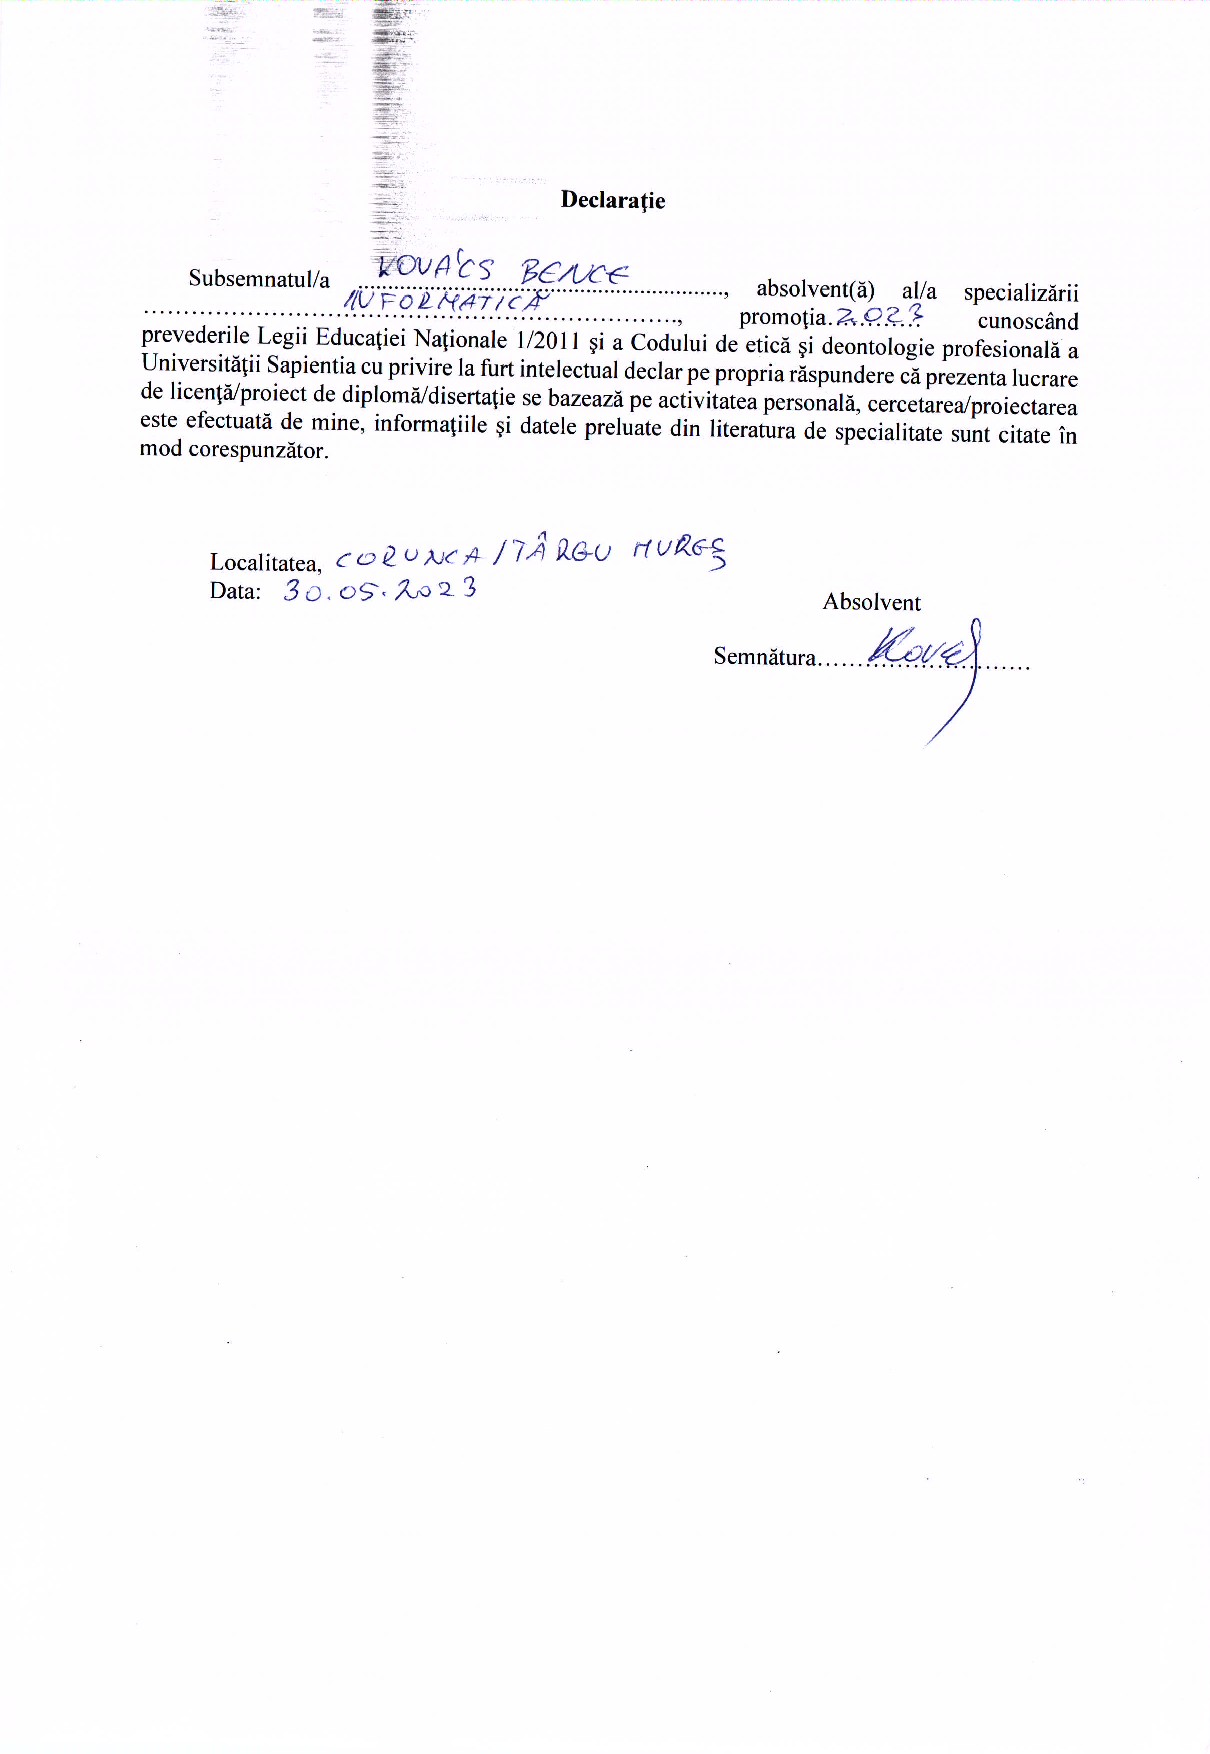
\includepdf[pages={1}]{content/Declaratie.pdf}
	\pagenumbering{gobble}

\selectlanguage{magyar}
\hungarianParagraph

%----------------------------------------------------------------------------
% Abstract in Hungarian
%----------------------------------------------------------------------------

\chapter*{Kivonat}

Napjainkban az online jegyvásárlás rohamos elterjedése figyelhető meg a technológia fejlődésével és az internet elérhetőségének növekedésével. Egy online platformon keresztül az emberek ma már kényelmesen és gyorsan tudnak jegyeket vásárolni különféle eseményekre, mint például koncertekre, színházi előadásokra vagy sporteseményekre, mint például a Formula-1.

Az online jegyvásárlás számos előnnyel jár. A vásárlók egyszerűen és kényelmesen böngészhetnek és választhatnak a széles körű jegyválaszték közül. Az online platformok részletes információkat nyújtanak az eseményekről, beleértve a dátumokat, helyszíneket és leírásokat. Emellett az online jegyvásárlás lehetővé teszi a jegyek összehasonlítását, árak és típusok kiválasztását, ami segít a vásárlóknak a legjobb lehetőség megtalálásában.

A technológiai fejlesztések, mint például a biztonságos online fizetési rendszerek és az elektronikus jegyek, hozzájárultak az online jegyvásárlás elterjedéséhez. A vásárlók könnyedén és biztonságosan fizethetnek az online platformokon (webshop) keresztül, és elektronikus jegyet kapnak, amelyet mobil eszközükön vagy nyomtatható formában mutathatnak fel az eseményen. Az online jegyvásárlás megkönnyíti az eseményekre való részvételt, hiszen a vásárlóknak nem kell hosszú sorokban állniuk a jegypénztáraknál. 


\vfill
\selectlanguage{romanian}

%----------------------------------------------------------------------------
% Abstract in Romanian
%----------------------------------------------------------------------------
\chapter*{Rezumat}

În prezent, se observă o răspândire rapidă a achiziționării de bilete online, odată cu dezvoltarea tehnologică și creșterea accesului la internet. Prin intermediul unei platforme online, oamenii pot cumpăra bilete confortabil și rapid pentru diverse evenimente, cum ar fi concerte, spectacole de teatru sau evenimente sportive, precum Formula 1.

Achiziționarea de bilete online vine cu numeroase avantaje. Cumpărătorii pot naviga și alege cu ușurință dintr-o gamă largă de opțiuni de bilete. Platformele online oferă informații detaliate despre evenimente, inclusiv date, locații și descrieri. De asemenea, achiziționarea de bilete online permite compararea prețurilor și selecționarea diferitelor tipuri de bilete, ceea ce ajută cumpărătorii să găsească cea mai bună opțiune.

Dezvoltările tehnologice, cum ar fi sistemele de plată online sigure și biletele electronice, au contribuit la răspândirea achiziționării de bilete online. Cumpărătorii pot plăti ușor și în siguranță prin intermediul platformelor online (webshop) și primesc biletele electronice, pe care le pot prezenta pe dispozitivele lor mobile sau sub formă printată la eveniment. Achiziționarea de bilete online facilitează participarea la evenimente, deoarece cumpărătorii nu mai trebuie să stea în rânduri lungi la casele de bilete.


\vfill
\selectlanguage{english}
%\englishParagraph

%----------------------------------------------------------------------------
% Abstract in English
%----------------------------------------------------------------------------
\chapter*{Abstract}

Currently, the rapid spread of online ticket purchasing can be observed due to technological advancements and the increased accessibility of the internet. Through an online platform, people can now conveniently and quickly purchase tickets for various events such as concerts, theater performances, or sports events like Formula 1.

Online ticket purchasing comes with numerous advantages. Customers can easily browse and choose from a wide range of ticket options. Online platforms provide detailed information about events, including dates, venues, and descriptions. Additionally, online ticket purchasing allows for ticket comparisons, price and type selections, which help customers find the best options available.

Technological developments, such as secure online payment systems and electronic tickets, have contributed to the widespread adoption of online ticket purchasing. Customers can easily and safely make payments through online platforms (webshop) and receive electronic tickets that can be presented on their mobile devices or in printable form at the event. Online ticket purchasing simplifies event attendance, as customers no longer have to wait in long queues at ticket counters.


\vfill
\dolgozatnyelve
\defaultParagraph
 
% Tartalomjegyzek
%~~~~~~~~~~~~~~~~~~~~~~~~~~~~~~~~~~~~~~~~~~~~~~~~~~~~~~~~~~~~~~~~~~~~~~~~~~~~~~~~~~~~~~
	\pagenumbering{arabic}
	\setcounter{page}{9}
	\tableofcontents\vfill

% A diplomadolgozat lenyegi resze
%~~~~~~~~~~~~~~~~~~~~~~~~~~~~~~~~~~~~~~~~~~~~~~~~~~~~~~~~~~~~~~~~~~~~~~~~~~~~~~~~~~~~~~

% ajánlott külön file-okba írni az egyes fejezeteket, ugyanis úgy jobban át lehet látni.

	%----------------------------------------------------------------------------
\addcontentsline{toc}{chapter}{Jelölések}
%----------------------------------------------------------------------------
\chapter*{Jelölések}

\begin{table}[h!]
	\centering
	\begin{tabular}{ | l | c | c | c | c |}
		\hline 
		\textbf{Rövidítés} & \textbf{Angol megnevezés} & \textbf{Magyar megnevezés}\\
		\hline
		F1 & Formula One & Formula-1/Forma-1\\
		\hline
		FIA & International Automobile Federation & Nemzetközi Automobil Szövetség \\
		\hline
		F1TM & F1 Ticket Manager & - \\
		\hline
		EDI & Electronic Data Interchange & Elektronikus Adatcsere \\
		\hline
		PDF & Portable Document Format & Hordozható Dokumentum Formátum \\
		\hline
		QR Code & Quick Response Code & Quick Response-kód (=gyors válasz) \\
		\hline
		E2EE & End-To-End Encryption & Végpontok Közötti Titkosítás \\
		\hline
		PIN & Postal Index Number & Postai Indexszám \\
		\hline
		DOM & Document Object Model & Dokumentum Objektum Modell \\
		\hline
		OSS & Open-Source Software & Nyílt Forráskódú Szoftver \\
		\hline
		NoSQL & Not only Structured Query Language & Nem csak Strukturált
		 Lekérdezőnyelv \\
		\hline
		API & Application Programming Interface & Alkalmazásprogramozási Felület \\
		\hline
		CDN & Content Delivery Network & Tartalomelosztó Hálózat \\
		\hline
		IDE & Integrated Development Environment & Integrált Fejlesztői Környezet \\
		\hline
		DBMS & Database Management Systems & Adatbázis-kezelő Rendszer (ABKR) \\
		\hline
		UI & User Interface & Felhasználói Felület \\
		\hline
		UX & User Experience & Felhasználói Élmény \\
		\hline
		HTML & HyperText Markup Language & Hiperszöveges Jelölőnyelv \\
		\hline
		CSS & Cascading Style Sheets & Lépcsőzetes Stíluslapok \\
		\hline
		HTTP & HyperText Transfer Protocol & Hiperszöveges Szállítási Protokoll \\
		\hline
		BCM & Block Cipher Mode & Blokktitkosítási Mód \\
		\hline
		AES & Advanced Encryption Standard & - \\
		\hline
		RSA & Rivest–Shamir–Adleman & - \\
		\hline
		REST & Representational State Transfer & - \\
		\hline
		MIT & Massachusetts Institute of Technology & Massachusettsi Műszaki Egyetem \\
		\hline
		\end{tabular}
		\label{tablazat1}
\end{table}

	%----------------------------------------------------------------------------
\chapter{Bevezető}%\addcontentsline{toc}{chapter}{Bevezető}
%----------------------------------------------------------------------------

\lstdefinelanguage{JavaScript}{
  keywords={
    typeof, new, true, false, catch, function, return, null, catch, switch, var,
    if, in, while, do, else, case, break, export, import
  },
  keywordstyle=\color{blue}\bfseries,
  ndkeywords={
    class, extends, const, let, constructor, super, static
  },
  ndkeywordstyle=\color{purple}\bfseries,
  identifierstyle=\color{black},
  sensitive=false,
  comment=[l]{//},
  morecomment=[s]{/*}{*/},
  commentstyle=\color{green}\ttfamily,
  stringstyle=\color{red}\ttfamily,
  morestring=[b]',
  morestring=[b]",
  literate=
    *{0}{{\textcolor{blue}{0}}}{1}
    {1}{{\textcolor{blue}{1}}}{1}
    {2}{{\textcolor{blue}{2}}}{1}
    {3}{{\textcolor{blue}{3}}}{1}
    {4}{{\textcolor{blue}{4}}}{1}
    {5}{{\textcolor{blue}{5}}}{1}
    {6}{{\textcolor{blue}{6}}}{1}
    {7}{{\textcolor{blue}{7}}}{1}
    {8}{{\textcolor{blue}{8}}}{1}
    {9}{{\textcolor{blue}{9}}}{1}
    {\ }{{ }}{1},
  keywords=[2]{random, PBKDF2, toString, stringify, encrypt, parse, decrypt},
  keywordstyle=[2]\color{green}\bfseries
}

\section {Témaválasztás indoklása}

Napjainkban az online jegyvásárlás nagy előretörést ért el a technológia fejlődésével az egyre szélesebb körben történő bankkártyás internetes vásárlások következtében. Egy online platformon keresztül az emberek ma már kényelmesen és gyorsan tudnak jegyeket vásárolni különféle eseményekre, mivel percek alatt el tudják végezni a világ bármely pontjából a nap bármely időpontjában. Az online jegyvásárlás számos előnnyel jár, amelyeknek köszönhetően egyre népszerűbbé válik.

Az egyik legfontosabb előny az online jegyvásárlás esetén az, hogy a vásárlók egyszerűen és kényelmesen böngészhetnek és választhatnak a széles körű jegyválaszték közül. Az online platformok részletes információkat biztosítanak az eseményekről, így a potenciális vásárlók teljes körű tájékoztatást kapnak az eseményről, mielőtt eldöntenék, hogy vásárolnak-e jegyet. Tehát a vásárlók magabiztosan dönthetnek arról, hogy melyik eseményre szeretnének jegyet vásárolni, anélkül, hogy bármilyen korlátozásba ütköznének.

A technológiai fejlesztések, mint például a biztonságos online fizetési rendszerek (\ref{abra:Logok}), amelyek az EDI rendszerek alkomponensei, és az elektronikus jegyek, hozzájárultak az online jegyvásárlás népszerűségéhez. A vásárlók könnyedén és biztonságosan fizethetnek az online platformokon keresztül, és elektronikus jegyet kapnak, amelyet mobil eszközükön vagy nyomtatható formában mutathatnak fel az eseményen. Az elektronikus jegyek további előnye, hogy nehezen veszíthetőek el vagy semmisülhetnek meg, így a vásárlók biztonságban tudhatják jegyeiket. Itt fontos megemlíteni, hogy ezen jegyek tárolása és biztonságban tartása további adatbiztonsági kérdéseket vet fel, amellyel foglalkozunk a dolgozat keretében. A platformokon keresztül a vásárlók egyszerűen választhatják ki a kívánt eseményt, a megfelelő ülőhelyet vagy jegytípust, és azonnal megvásárolhatják a jegyüket néhány kattintással. Ez időt és energiát takarít meg a vásárlók számára, ami napjainkban egy lényeges tényező.

\begin{figure}[!h]
	\centering
	
\includegraphics[scale=0.2]{images/logok}
	\caption{Online fizetési rendszerek}
	\label{abra:Logok}
\end{figure}
\pagebreak

További előnyeként egy ilyen platformnak megemlítendő, hogy a szervezők számára is jelentősen hatékonyabbá teszi a rendelések nyomon követését, statisztikák készítését, amelyeket felhasználhatnak értékesítési jelentések és a marketing javításához. Emellett az online jegyvásárlás lehetőséget nyújt a szervezőknek arra is, hogy célzottan reklámozzák az eseményüket, így nagyobb látogatottságot érhetnek el.

A jelenleg is működő hivatalos platform, ahol direkt módon juthatunk hozzá jegyekhez az FIA Formula-1-es versenyhétvégékre, az F1 Experiences. Itt gyorsan és kényelmesen vásárolhatjuk meg a kívánt jegyünket, amelyet a sikeres rendelés és kifizetés után emailben kapjuk meg PDF formátumban, amely tartalmazza a megvásárolt jegy(ek)et, egyedi azonosítókat, QR kódokat és a számlázási adatokat. Az eseményre érve, a belépő kapuknál, egy erre a célra kihelyezett okos eszközzel megtörténik a QR kód olvasása és hitelesítése. Pozitív eredmény esetén beléphetünk az esemény helyszínére.

A fent említett folyamat megengedi, hogy ezek az elektronikus jegyek átruházhatóak a tulajdonos által bárki számára. Ezzel persze önmagában nincs probléma, mivel ezt a szabadságot meg kell lehessen adni a felhasználóknak, hogy bizonyos esetekben más személy tudjon részt venni a vásárló helyett, így nem vész kárba a vásárlás. Ez a rendszer viszont teret ad egy olyan biztonsági kérdésnek, amelyet jelenleg a felhasználó felelősségére van bízva, miszerint ezt a kódot akár hetekkel, hónapokkal a használatuk előtt kapnak meg a felhasználók elektronikus levél formájában és azt bárki megszerezheti, akinek hozzáférése van a fiókhoz. Rosszabb esetekben, egy szándékos kibernetikai támadás esetén is eltulajdoníthatják és felhasználhatják. Ennek persze kisebb a valószínűsége, viszont ami egy aggasztó tény, hogy a felhasználók nagy része nem megfelelő módon kezeli az adatainak a biztonságos tárolását és számos esetben fellelhetőek olyan emberi hibák, amelyeket kihasználnak az adathalászok, hogy hozzáférjenek a megvásárolt jegyekhez és saját célokra használják fel, többnyire illegális módon kereskedjenek velük.

\pagebreak
Gyakran megtörténik, hogy egy felhasználó több oldalra is ugyanazokat a bejelentkezési adatokat adja meg a regisztráció során. Ez többségében a személyes email fiók felhasználó nevével és jelszavával megegyezik és ezt az adathalászok is figyelembe veszik. Egy másik sebezhetőség, hogy számos esetben egy fiókhoz több személy is hozzáfér, így már nem beszélhetünk biztonságos adattárolásról. Megemlítendő viszont, hogy az email szolgáltatók biztosítanak E2EE-t az elektronikus levelek küldésekor és fogadásakor.

Az F1 Ticket Manager webes alkalmazás célja az alapvető jegyvásárlási funkcionalitások biztosítása, valamint a teljes vásárlási folyamat biztonságosabbá tétele. Ennek megvalósítására számos technológiai fejlesztés és programozói technika létezik. Az alkalmazás fejlesztésénél beépítésre került PIN kódok használata, amely egy emelt szintű biztonságot nyújt a felhasználó számára, valamint egy titkosítási algoritmus, amely az eredeti adatok azonnali visszafejtését hivatott megnehezíteni. 

	%----------------------------------------------------------------------------
\chapter{Rendszerspecifikáció} \label{fejezet3}
%----------------------------------------------------------------------------

\section {Rendszer követelmények}

A rendszer specifikációit négy nagy részre oszthatjuk fel, amelyek közé tartoznak a felhasználói felület-, a jegyvásárlás-, a felhasználók- és a biztonság specifikációja. Elsőként a felhasználói felület biztosítja a felhasználó és a rendszer közötti kommunikációt. A jegyvásárlás a rendszer központi funkcionalitása, ezáltal a legkomplexebb is. Az alkalmazás lehetővé teszi a több típusú felhasználók hozzáférését a különbőző funkcionalitásokhoz. Végül de nem utolsó sorban a rendszer a bizalmas adatok biztonságát is hivatott kiszolgálni. A specifikációk prezentálására a Visual Paradigm Online felület segítségével hoztam létre a szükséges diagramokat \cite{VPO}. A rendszer működését vizsgálni tudjuk a funkcionális- és nem funkcionális követelmény alapján.
\subsection {Funkcionális követelmények} \label{rendszerFunkcionális}

A funkcionális követelmények a rendszer funkcionalitásaira vonatkoznak, azaz meghatározzák, hogy milyen feladatokat és műveleteket kell elvégeznie a rendszernek, milyen funkciókat kell biztosítania a felhasználók számára.

\begin{itemize}
  	\item[\textbf{a,}] \textbf{Felhasználói szerepkörök:}

Az oldal böngészésének tekintetében érdemes különboző jogosultságokkal rendelkező szerepköröket kialakítani. Erre azért van szükség, mivel a rendszer több típusú felhasználó által látogatható. Ezek közül a legelső és egyben a legkevesebb funkcionalitással rendelkező az \textbf{Anonymous}, amelyek \textit{be nem jelentkezett} felhasználók, esetében ilyen funkcionális követelmények például a jegyek közötti böngészés lehetősége, a jegyek részleteinek megtekintése, valamint az email-küldés a \textit{Support} számára. Emellett fontos, hogy az Anonymous felhasználók be tudjanak jelentkezni az oldalra vagy új felhasználói fiókot tudjanak regisztrálni, és ez a bejelentkezési folyamat lehetőséget biztosít az oldalon regisztrált fiókok vagy akár más közösségi fiókok használatára is (\ref{abra:useCaseNA}).

\begin{figure}[!h]
	\centering
	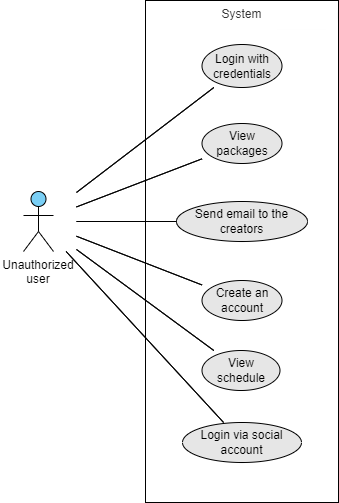
\includegraphics[scale=0.7]{images/useCaseNA}
	\caption{Use case diagram - Nem bejelentkezett felhasználó}
	\label{abra:useCaseNA}
\end{figure}
\pagebreak

A \textbf{Regular} felhasználók esetében elvárt, hogy \textit{be legyenek jelentkezve} a rendszerbe. Lehetőségük van a jegyek kosárba helyezése, visszajelzések írása és jegyek értékelése. Emellett a felhasználók képesek megtekinteni a profiljukat, ahol lehetőségük van felhasználói név és profil kép változtatására, valamint a vásárlási előzményeik megtekintésére. Az előzmények részleteinél a felhasználóknak lehetőségük van az adott jegy PIN kódjának megváltoztatására, amennyiben szükséges. A vásárlási folyamat során a felhasználók a rendelési oldalra (\textit{Checkout}) jutnak el, ahol lehetőségük van a listaelemek mennyiségének módosítására vagy azok törlésére. Itt történik meg a fizetés és a rendelés leadása (\ref{abra:useCaseA}).

\begin{figure}[!h]
	\centering
	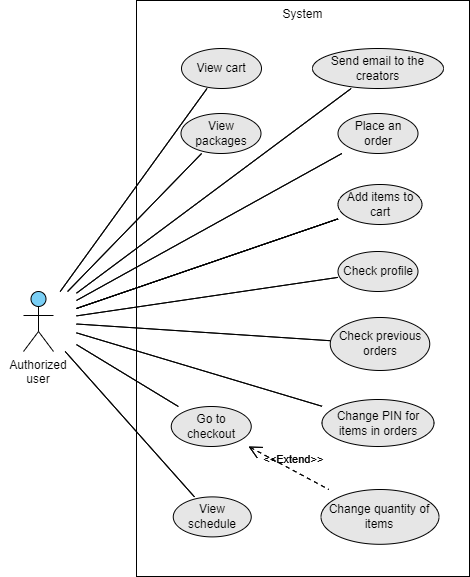
\includegraphics[scale=0.7]{images/useCaseA}
	\caption{Use case diagram - Bejelentkezett felhasználó}
	\label{abra:useCaseA}
\end{figure}
\pagebreak

Az adminisztrátorok a harmadik kategóriát alkotják a rendszerben, és különleges jogosultságokkal rendelkeznek. Az \textbf{Admin} felhasználóknak joguk van az összes korábban említett funkcionalitáshoz, mint például a jegyek kosárba helyezése, visszajelzések írása és értékelése, valamint a profiljuk kezelése és vásárlási előzményeik megtekintése. Azonban az Admin felhasználóknak további feladatuk is van, nevezetesen a jegyek hitelesítése.

Az Admin felhasználóknak lehetőségük van a jegyek hitelesítésére, amelyhez a QR kódot be kell olvasniuk és meg kell adniuk a PIN kódot. Ez a folyamat biztosítja, hogy csak érvényes jegyek kerüljenek elfogadásra és használatra a rendszerben. Ez a szerepkör manuálisan adható hozzá a rendszerhez, és szükség esetén módosítható.

Fontos megjegyezni, hogy bár az adminisztrátoroknak lehetőségük van jegyek vásárlására, ezt kizárólag a rendszer tesztelésére és karbantartására szolgáló célokra használható. Az adminisztrátorok elsődleges felelőssége a rendszer megfelelő működésének biztosítása és a jegyek hitelesítése (\ref{abra:useCaseAdmin}).

\begin{figure}[!h]
	\centering
	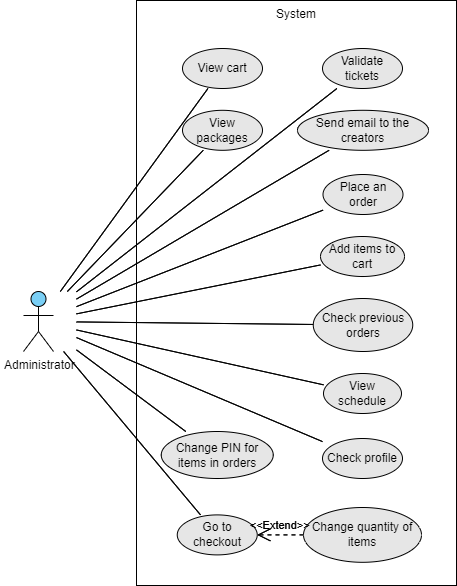
\includegraphics[scale=0.7]{images/useCaseAdmin}
	\caption{Use case diagram - Adminisztrátor}
	\label{abra:useCaseAdmin}
\end{figure}
\pagebreak

  	\item[\textbf{b,}] \textbf{Jegyvásárlás:}

A \textbf{jegyvásárlás} során a felhasználóknak számos funkcionalitást kell biztosítani. Először is, lehetőséget kell adni nekik, hogy kiválaszthassák a jegyeket és azokat kosárba helyezhessék. Emellett fontos, hogy a felhasználók módosíthassák a jegyek mennyiségét vagy akár törölhessék azokat, ha szükséges. A böngészés során pedig lehetővé kell tenni számukra, hogy részletes információkat kapjanak a jegyekről, mint például a helyszín, az időpont vagy az ár. Ez segíti őket a megfelelő döntéshozatalban és a kívánt jegyek megtalálásában.


  	\item[\textbf{c,}] \textbf{Bejelentkezés és regisztráció:}

A \textbf{bejelentkezés} és \textbf{regisztráció} lehetővé teszik a felhasználók számára, hogy saját profiljuk legyen a rendszerben, amellyel vásárlásokat tudnak végrehajtani és nyomon tudják követni azokat.

A \textbf{bejelentkezés} folyamata magában foglalja a felhasználónév és jelszó megadását vagy egy harmadik féltől származó fiók segítségével. A felhasználóknak lehetőségük van megadni a regisztrált felhasználónevüket és a hozzájuk tartozó jelszavukat a bejelentkezéshez. A felhasználói felületnek tartalmaznia kell egy bejelentkezés gombot, amelyre kattintva a felhasználó bejelentkezik a rendszerbe. Ezután a rendszer ellenőrzi az adatok helyességét és hitelesíti a felhasználót, hogy hozzáférjen a felhasználói funkciókhoz.

A \textbf{regisztráció} lehetőséget ad a felhasználóknak arra, hogy új fiókot hozzanak létre a rendszerben. Ehhez a felhasználóknak kitöltetniük kell egy regisztrációs űrlapot, amely tartalmazza az szükséges adatokat, például felhasználónevüket, jelszavukat, e-mail címüket. A felületnek tartalmaznia kell egy regisztrációs gombot, amelyre kattintva a rendszer regisztrálja a felhasználót és létrehozza az új fiókját.
\end{itemize}

\subsection {Nem funkcionális követelmények}

A nem funkcionális követelmények olyan aspektusokra fókuszálnak, amelyek nem közvetlenül a rendszer funkcionalitásához kapcsolódnak, hanem inkább annak működési jellemzőit, tulajdonságait vagy környezeti tényezőit érintik.

\begin{itemize}
  	\item[\textbf{a,}] \textbf{Felhasználói szerepkörök:}

A \textbf{felhasználói szerepkörök} között egyértelmű határvonal kell legyen, hogy melyeknek mihez van jogosultságuk. A felhasználóknak könnyen és zökkenőmentesen kell tudniuk használni az oldalt függetlenül a szerepkörüktől. Fontos továbbá, hogy az egyes szerepkörökhöz tartozó jogosultságok és hozzáférési szintek megbízhatóak és biztonságosak legyenek, hogy a felhasználók csak azokhoz az információkhoz és funkciókhoz férjenek hozzá, amelyek az adott szerepkörhöz kötött.

 	 \item[\textbf{b,}] \textbf{Jegyvásárlás:}

A \textbf{jegyvásárlási} folyamatnak gyorsnak és hatékonynak kell lennie. A rendszernek képesnek kell lennie a nagyobb mennyiségű jegykezelésre és skálázhatónak kell lennie, hogy a jegyvásárlás során ne jelentkezzenek teljesítménybeli problémák. Emellett a jegyvásárlás folyamatának biztonságosnak is kell lennie, és megfelelő védelmi intézkedéseket kell tartalmaznia az adatbiztonság érdekében. Ilyen intézkedések például a titkosított adatátvitel vagy a vásárlói adatok megfelelő védelme.

	 \item[\textbf{c,}] \textbf{Bejelentkezés és regisztráció:}

A \textbf{bejelentkezés és regisztráció} folyamata kapcsán a nem funkcionális követelmények között szerepel, hogy a folyamatnak biztonságosnak kell lennie. A bejelentkezési és regisztrációs folyamatnak megfelelő hitelesítési és azonosítási mechanizmusokat kell tartalmaznia. Emellett a folyamatnak gyorsnak és felhasználóbarátnak kell lennie, hogy a felhasználók könnyedén és zökkenőmentesen tudjanak bejelentkezni vagy regisztrálni. A felhasználóknak egyszerű és intuitív felhasználói felületet kell biztosítani a bejelentkezéshez és regisztrációhoz, hogy könnyen megadhassák szükséges információikat és végrehajthassák az adott folyamatot.
\end{itemize}


\section {Felhasználói követelmények}

\begin{itemize}
  	\item[\textbf{a,}] \textbf{Funkcionalitások:}

A főbb funkcionalitások tervezésénél, amelyekről szó volt a funkcionális rendszer követelmények alfejezet (\ref{rendszerFunkcionális}) keretében, figyelembe vettem, hogy azok a lehető legjobban betöltség a feladatukat, így a felhasználók zökkenőmentesen tudják használni a rendszert. Figyelembe vettem az implementáció során a funkcionalitások teljesítményének, megbízhatóságának és használhatóságának a fontosságát.

	\item[\textbf{b,}] \textbf{Felhasználói felület:}

A rendszer felhasználói felületének fejlesztése első sorban arra irányult, hogy intuitív és könnyen érthető legyen, ezáltal a felhasználók ne tapasztaljanak nehézségeket vagy zavarokat az alkalmazás használata során. Egy felhasználó első benyomása határozza meg a legnagyobb mértékben a rendszerről alkotott véleményét, ezért kellő figyelmet fordítottam arra, hogy az oldal letisztult legyen, elkerülve a félrevezető utasításokat és funkcionalitásokat. A felhasználó az oldal első látogatásakor értesül az oldal céljáról és további információkról a hivatalos oldalak elérésére.

	\item[\textbf{c,}] \textbf{Teljesítmény és megbízhatóság:}

Az alkalmazás teljesítménye több komponensből áll össze, amelyek közé tartoznak a reakcióidő, válaszkészség, stabilitás és rendelkezésre állás. Fontosnak tartottam, hogy az alkalmazás gyorsan és megbízhatóan működjön, hogy a felhasználók ne érezzenek frusztráló lassulásokat vagy hibákat. Persze a hibák teljes mértékű elkerülése majdnem hogy lehetetlen a szoftver rendszerek esetében, mivel az emberi hiba lehetősége mindig jelen van. Arra törekedtem, hogy minimalizálva legyen a hibák előfordulásának lehetősége és megelőző intézkedéseket vezettem be. Ide tartoznak azok a megfelelő hibaüzenet is, amelyek kisebb vagy nagyobb hibák esetén is célravezető módon informálják a felhasználót, hogy ez a hiba miként folyásolja be a rendszer további működését vagy adott esetben mit tud tenni a felhasználó a hiba elkerülése ellen.

	\item[\textbf{d,}] \textbf{Profilkezelés:}

A felhasználók számára fontos szempont, hogy hozzáférjenek a saját adataikhoz egy oldalon és modosítani tudják őket. Erre a célra hoztam létre egy aloldalt, ahol kényelmesen lehet profil képet, felhasználónevet módosítani és a rendelési előzmenyeket visszanézni. Továbbá lehetőségük van, hogy az egyes rendelésekhez új PIN kódot rendeljenek.

	\pagebreak
	\item[\textbf{e,}] \textbf{Kompatibilitás:}

Az alkalmazás elsősorban a desktop számítógépekre lett optimalizálva, viszont egy következő továbbfejlesztési lehetőség lenne, hogy reszponzív legyen, ezáltal mobilon és táblagépen kezelhetőbb. A rendszer kompatibilis a közismert modern böngészők mindegyikével, mint a Microsoft Edge, Google Chrome, Mozilla Firefox, Apple Safari vagy az Opera (\ref{abra:browserLogos}).

\begin{figure}[!h]
	\centering
	
\includegraphics[scale=0.2]{images/browserLogos}
	\caption{Web böngészők}
	\label{abra:browserLogos}
\end{figure}
\end{itemize}
	%----------------------------------------------------------------------------
\chapter{A rendszer architektúrája}
%----------------------------------------------------------------------------

Az alkalmazás architektúrája három nagyobb komponensből áll. Mindhárom egy különálló szerver, amelyek egy összefüggő gráfként képesek kommunikálni egymással (\ref{abra:architecture}).

\begin{figure}[!h]
	\centering
	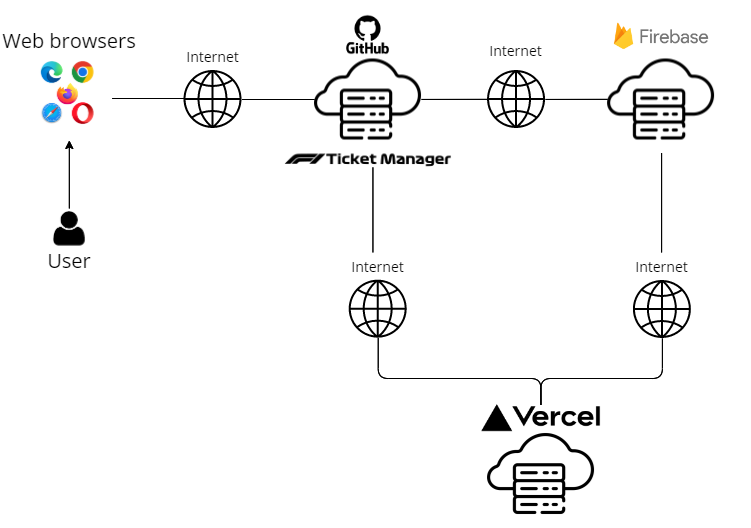
\includegraphics[scale=0.7]{images/architecture}
	\caption{Rendszer architekúra}
	\label{abra:architecture}
\end{figure}

Az rendszer fő komponense a weboldalt üzemeltető szerver, a \textbf{GitHub Pages}. Ez felel az oldal rendereléséért és valós időben elérhetőségéről. Erre azért van lehetőség, mivel a forráskód megtalálható a GitHub-on, amelyet összekötöttem a GitHub Pages-el. A deployment fázis során a GitHub egy optimalizált kódot generál és azt hosztolja \cite{Deploy}.

A második komponens a \textbf{Google Firebase} CDN alapú felhőalapú szolgáltató. Segítségével meg lehet valósítani felhasználók autentikációját, adatok tárolását egy NoSQL adatbázis-kezelő rendszerben és még sok mást. Azért ezeket emeltem ki, mivel ezek a funkcionalitások játszanak szerepet a rendszerben. A weboldal folyamatosan kommunikál a Google Firebase-el, hogy valós időben és hatékonyan tudja kiszolgálni a felhasználókat. Az \textbf{F1 Ticket Manager} egyik központi eleme a jegyek kezelése, amely során titkosítási algoritmusok futnak a felhasználók adatainak biztonsága érdekében. Mivel ezeket az algoritmusokat nem lehetséges, hogy a Google Firebase ingyenes verziójával igénybe vegyem, ezért szükségem volt egy másik backend szerverre is, ahol el tudom végezni ezeket a műveleteket.

A harmadik és egyben utolsó komponens a \textbf{Vercel} felhőalapú szolgáltató, amelyen fut egy NodeJs szerver, amelyet én fejlesztettem. Ennek a szervernek a API-jai felelnek a titkosítási folyamatokért. Mivel az adatok csak a {Google Firestore}-ban vannak tárolva, ezért elengedhetetlen, hogy kommunikáljon vele. 

\section {GitHub frontend architektúra} \label{frontend}

A rendszer frontendjét szolgáló komponens, amelyet a GitHub Pages hosztol, egy \textbf{create-react-app} alkalmazás. Ez egy olyan \textbf{npm} (\ref{abra:npmLogo}) JavaScript futási környezet csomagkezelője \cite{WikiNpm} által forgalmazott projekt sablon, amely tartalmazza az alapvető konfigurációkat és fájlokat, amelyek szükségesek egy \textbf{React} alkalmazás készítéséhez.

\begin{figure}[!h]
	\centering
	
\includegraphics[scale=0.2]{images/npmLogo}
	\caption{Az npm csomagkezelő}
	\label{abra:npmLogo}
\end{figure}

Az F1TM frontend kódbázisának gyökérkönyvtára az \textit{src} mappa (\ref{abra:srcFolderStructure}), amely tartalmazza az alkalmazás komponenseit, oldalait, a többi szerver végpontjaira kapcsolódó függvényeket és a React \textbf{Redux} kezelésére használt kódokat.

\begin{figure}[!h]
	\centering
	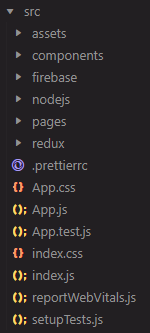
\includegraphics[scale=0.6]{images/srcFolderStructure}
	\caption{Az src mappa struktúrája}
	\label{abra:srcFolderStructure}
\end{figure}

A mappa struktúrába rendezett komponensek (\ref{abra:components}) áttekinthetőbbé teszik a rendszert. Az adott funkcióhoz tartozó összes fájl vagy modul egy helyen vannak, így könnyen megtalálhatóak és karbantarthatóak. Ez különösen hasznos, ha több fejlesztő dolgozik ugyanazon a rendszeren, vagy ha idővel vizsgálni vagy módosítani kell a komponenseket.

Az alaposan megszervezett struktúra lehetővé teszi a komponensek könnyű újrafelhasználását. Ez jelentősen csökkentheti a fejlesztési időt és erőforrásokat, mivel nem kell mindent újra implementálni vagy átírni.

Továbbá egy új funkció bevezetésénél nagyon megkönnyíti a mapparendszer, hogy könnyen megtaláljam a megfelelő helyét az új fájloknak. Az új funkciót egy új komponensként hozzáadhatjuk a megfelelő mappába anélkül, hogy át kellene írni vagy megváltoztatni a meglévő komponenseket. Ez tisztább és kevésbé összezavaró kódbázist eredményez, és minimalizálja a mellékhatásokat vagy a hibák kockázatát.

\begin{figure}[!h]
	\centering
	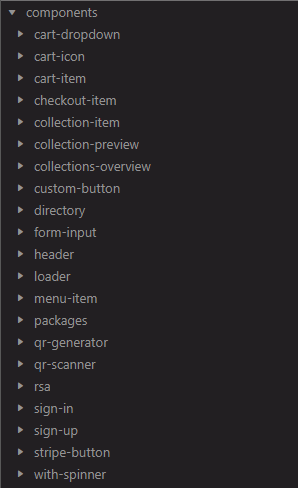
\includegraphics[scale=0.6]{images/components}
	\caption{Komponensek}
	\label{abra:components}
\end{figure}

A \textbf{Vercel} szerverrel való kommunikációra az \textbf{axios} csomagot használtam. Ennek segítségével tudom kezelni a hálózaton történő HTTP kéréseket, amelyekhez hozzátartozik az url, body és egyéb paraméterek megadása.

\section {Google Firebase backend architektúra} \label{firebase}

A \textbf{Google Firebase} olyan platform, amely lehetővé teszi a fejlesztők számára, hogy könnyedén építsenek és üzemeltessenek felhőalapú alkalmazásokat. A Firebase architektúrája több szolgáltatásból áll, amelyek együttműködnek, hogy biztosítsák a fejlesztők számára a skálázhatóságot, megbízhatóságot és az alkalmazások széleskörű funkcióit (\ref{abra:firebaseConsole}).

A Google Firebase funkcionalitásainak elérésére léteznek direkt JavaScript alapú keretrendszerekre könyvtárcsomagok. ReactJs-re a \textit{firebase} és annak almoduljai a \textit{/storage}, \textit{/compat/app}, \textit{/compat/auth} vagy a \textit{/compat/firestore}, míg NodeJS-ben a \textit{firebase-admin}. Ezekben a modulokban implementálva minden kérés a Firebase felé és a visszakapott adatok deszerializálása. Például a \textbf{storage} modullal lehetséges a Cloud Storage kezelése és az \textbf{auth}-al a felhasználók bejelentkeztetése és az adataik kezelése.

\begin{figure}[!h]
	\centering
	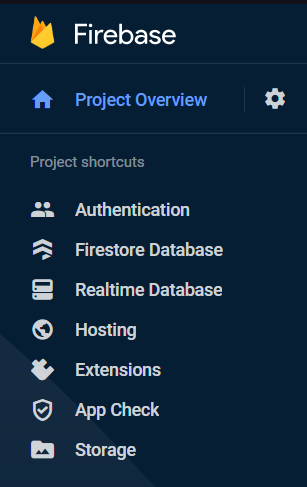
\includegraphics[scale=0.6]{images/firebaseConsole}
	\caption{Firebase Console}
	\label{abra:firebaseConsole}
\end{figure}
\pagebreak

\subsection {Firebase Authentication}

A rendszeremben az egyik központi szerepet játszó szolgáltatás a \textbf{Firebase Authentication}. Ennek segítségével a felhasználók regisztrálhatnak, bejelentkezhetnek és hitelesíthetik magukat az alkalmazásban. Ez a szolgáltatás támogatja az email-alapú, és közösségi média alapú hitelesítési módokat is, és lehetővé teszi a felhasználói adatok kezelését. Az F1 Ticket Managerben lehetőség van regisztrálni email cím, Google vagy Facebook fiók segítségével (\ref{abra:loginMethods}). Amennyiben saját email fiókkal történik a regisztráció, szükség van annak vissza igazolására, amely a megadott fiókra érkező levélben megadott linkkel lehetséges.

\begin{figure}[!h]
	\centering
	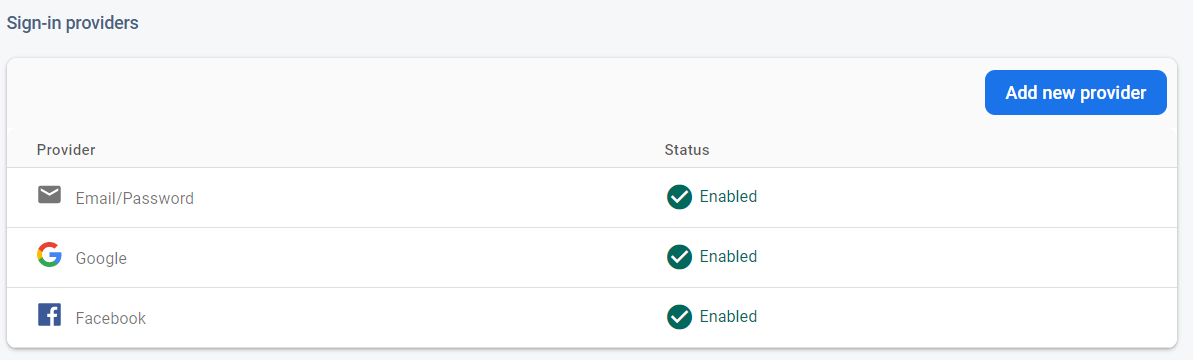
\includegraphics[scale=0.4]{images/loginMethods}
	\caption{Autentikációs módok}
	\label{abra:loginMethods}
\end{figure}

A \ref{firebase} fejezetben is említett \textit{/compat/auth} modul által lehetőségem van a rendszer bármely pontján elérni az aktuálisan bejelentkezett felhasználó adatait a \textit{firebase.currentUser}-en keresztül.

\subsection {Cloud Firestore}

A második, általam leghasználtabb, funkcionalitás a \textbf{Cloud Firestore}. A Firestore egy dokumentum-orientált adatbázis, amely skálázhatóbb és rugalmasabb lehetőségeket kínál adatok tárolására és lekérdezésére. Firestore használatakor a fejlesztők strukturált gyűjteményeket és dokumentumokat hozhatnak létre, és lehetőségük van komplex lekérdezések végrehajtására és az adatok szűrésére. Ilyen dokumentumokban tárolom a felhasználói adatokat, amelyek nagyrésze meg is jelenik a felületen, a pályák és jegyek adatait, valamint a rendeléseket (\ref{abra:firestoreStructure}). A pályaadatokat egy JSON fájlban gyűjtöttem össze és abba lehetséges a módosításuk is, majd egy általam írt kód segítségével ebből a JSON adatcsomagból létrehozok egy többrétegű dokumentumrendszert a Firestoreban.

\begin{figure}[!h]
	\centering
	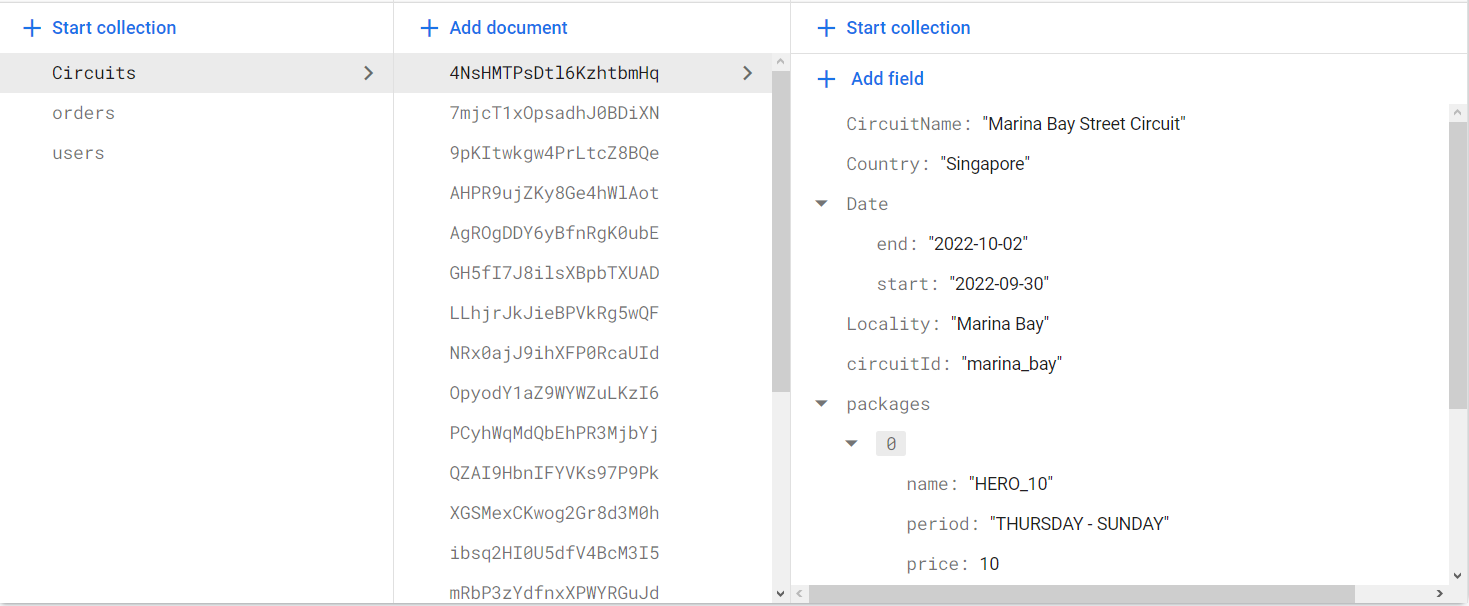
\includegraphics[scale=0.4]{images/firestoreStructure}
	\caption{Cloud Firestore struktúrája}
	\label{abra:firestoreStructure}
\end{figure}

A adatbázis megfelelő biztonságát a \textbf{szabályok} (Rules) beállításával lehet megadni. Ezen szabályok tudják biztosítani, hogy az adott dokumentumokhoz milyen feltételek alapján lehet hozzáférni. Ilyen például, hogy egy felhasználó adataihoz mindig csak a \textit{Firebase Authentication} által bejelentkezett felhasználó férjen hozzá az egyedi azonosító alapján (auth.uid) (\ref{code:databaseRules}).

\begin{lstlisting}[caption={Firestore szabályok.}, captionpos=b, label={code:databaseRules}]
match /databases/{database}/documents {
    match /users/{userId} {
      // Allow users to only read or write their own documents
    	allow read, write: if request.auth.uid == userId;
    }
}
\end{lstlisting}

\subsection {Firebase Storage}

A \textbf{Firebase Storage} szolgáltatás lehetővé teszi a felhasználói fájlok, például képek, videók vagy hangfájlok tárolását és kezelését. A Firebase Storage nagyobb méretű fájlok tárolására és letöltésére specializálódott, amelyeket a Google Cloudban tárolja. Az én alkalmazásomban a feltöltött profilképek kerülnek a Storage-ban tárolásra (\ref{abra:storageStructure}).

\begin{figure}[!h]
	\centering
	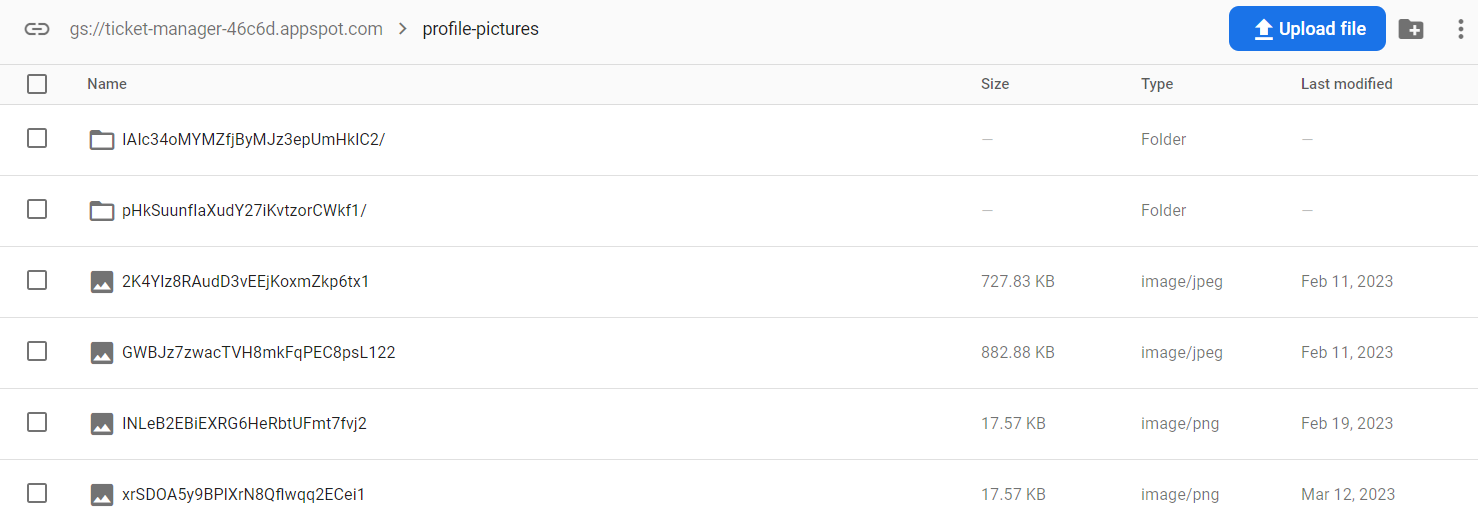
\includegraphics[scale=0.4]{images/storageStructure}
	\caption{Firebase Storage struktúrája}
	\label{abra:storageStructure}
\end{figure}
\pagebreak

\section {Vercel backend architektúra}

A \textbf{Vercel} által kiszolgált egyik backend szerver, amely hasonlóan a frontendhez (\ref{frontend}) JavaScript nyelven van írva \textbf{NodeJS} keretrendszerben (\ref{abra:vercelStructure}). A szerver kiinduló pontja az \textit{app.js}, amely tartalmazza az alapértelmezett konfigurációkat a HTTP hívások kezelésére és a végpontokat tartalmazó fájlok helyét. A szerver textbf{Express} alapú.

A Vercel-en több sablon alapján lehet szervert létrehozni. Én egy egy third-party repository segítségével hoztam létre, amely megtalálható a GitHubon a \textbf{geshan} nevű felhasználó jóvoltából \cite{GitNodeSql}.

Az Express.js, vagy egyszerűen csak Express, egy backend webalkalmazás-keretrendszer RESTful API-k létrehozásához a Node.js segítségével, amelyet ingyenes és nyílt forráskódú szoftverként adnak ki az MIT-licenc alatt \cite{WikiExpress}.

\begin{figure}[!h]
	\centering
	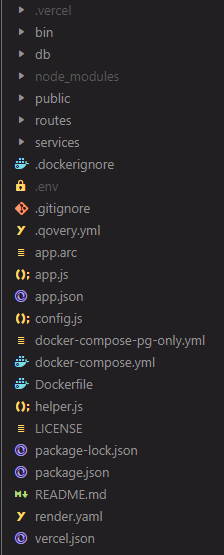
\includegraphics[scale=0.6]{images/vercelStructure}
	\caption{Vercel mappa struktúrája}
	\label{abra:vercelStructure}
\end{figure}

A \textbf{routes} mappa tartalmazza a alkalmazás működéséhez szükséges JSON, CSS és egyéb JS fájlokat. Az én esetemben itt találhatóak az \textit{index.js} és a \textit{quotes.js} fájlok (\ref{abra:vercelRoutes}). Az index.js tartalmazza a szerver végpontjait és az üzleti logikát. A quotes.js pedig a Google Firebase szerverrel való kapcsolat kialakításához szükséges konfigurációkat, amelyek lefutnak a szerver indulásakor.

\begin{figure}[!h]
	\centering
	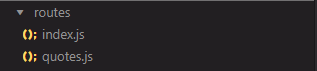
\includegraphics[scale=0.8]{images/vercelRoutes}
	\caption{Vercel \textit{Routes} mappa}
	\label{abra:vercelRoutes}
\end{figure}

A titkosítási és kulcscsere algoritmusok használatára rendre a \textbf{crypto-js} és \textbf{node-rsa} JavaScript könyvtárcsomagokat használom \cite{NRSA} \cite{CJS}. A node-rsa egy optimális és kényelmes használatot nyújt az RSA publikus kulcscsere protokoll beépítéséhez a rendszerbe. Ez egy emelt szintű biztonságot biztosít a felhasználók számára. Azt is figyelembe vettem, hogy ez a kulcscsere csak akkor biztonságos, ha a kulcsokat is biztonságos módon tároljuk. Erre azt a megoldást alkalmaztam, hogy a publikus és privát kulcsokat is a Google Firestore-ban tárolom, amelyre olyan szabályok (rules) vannak beállítva, hogy mindig csak az adott autentikált felhasználó férjen hozzá, ahogyan arról már említést tettem a \ref{firebase} fejezetben a \ref{code:databaseRules} kódrészlet segítségével.
	%----------------------------------------------------------------------------
\chapter{Tervezés és megvalósítás}
%----------------------------------------------------------------------------

A rendszer architektúrájának tervezése során figyelembe vettem a \ref{research}. és \ref{scopes}. fejezetekben kitűzött célokat. Az eredeti tervek elkészültével kezdetét vette a megvalósítás. Az implementáció során felmerültek olyan akadályok és újabb ötletek, amelyek kisebb-nagyobb mértékben befolyásolták a terveket. Erre számítottam és éppen ezért úgy próbáltam tervezni, hogy dinamikusan módosíthatóak legyenek bővítés vagy módosítás esetén. A tervezési és megvalósítási folyamat hónapokat vedd igénybe annak érdekében, hogy minden jelentkező problémát és az újabb ötleteket legyen idő átgondolni.

\section {Az alkalmazás frontendje}

\subsection {Kezdőoldal (Homepage)}

Tekintettel arra, hogy az alkalmazás bizonyos funkcionalitásai használhatóak bejelentkezés nélkül is, a kezdőoldal egy üdvözlő oldal egy navigációs menüvel az oldal tetején. Amennyiben egy eszközről első alkalommal lépik az oldalra egy felhasználó, akkor egy információs ablakkal találkozik \cite{Modal}, amely tartalmazza az alkalmazás célját, a hivatalos forrásokat a jegyvásárlásra és ezeknek a jogtulajdonosait (\ref{abra:homepagePopup}).

Annak érdekében, hogy ez az ablak csak egyszer jelenjen meg \textbf{sütiket (Cookies)} használok. Ezek a sütiket a böngésző tárolja a felhasználó eszközén és a weboldal betöltésekor a böngésző betölti az elmentett sütiket, ha vannak. Ezek kulcs-elem párok, amely értelmében egy tetszőleges nevű kulcs alatt tudok elmenteni majdnem bármilyen adatot. Ha a felhasználó rákattint az \textbf{Understood} gombra, akkor egy \textbf{modalAccepted} kulcs alatti sütiben eltárolom a \textbf{true} értéket és amikor betöltődik az alkalmazás ezt az értéket ellenőrzöm.
Mint említettem ezek a sütik lokálisan vannak tárolva a felhasználónál és ha a felhasználó kitörli azokat, amelyek ehhez az oldalhoz tartoznak, akkor egyértelműen újra elő fog jönni az ablak.

\begin{figure}[!h]
	\centering
	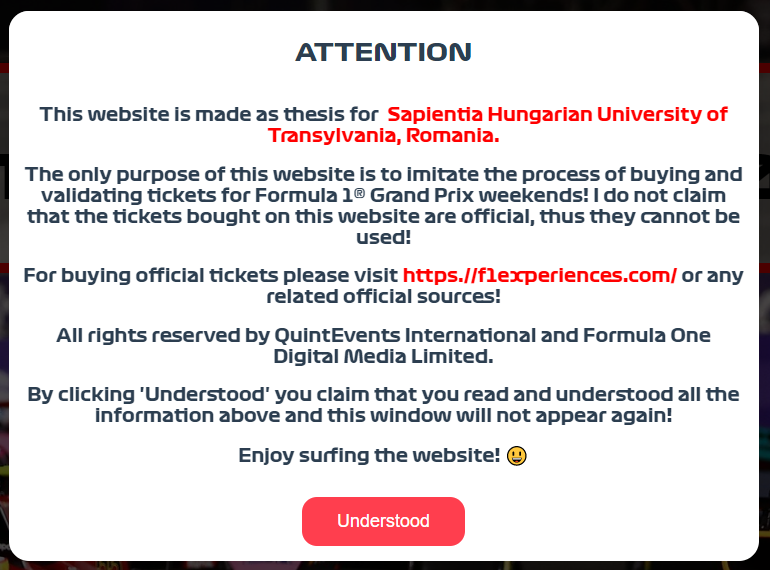
\includegraphics[scale=0.4]{images/homepagePopup}
	\caption{Kezdőoldalon felugró ablak}
	\label{abra:homepagePopup}
\end{figure}
\pagebreak

\begin{figure}[!h]
	\centering
	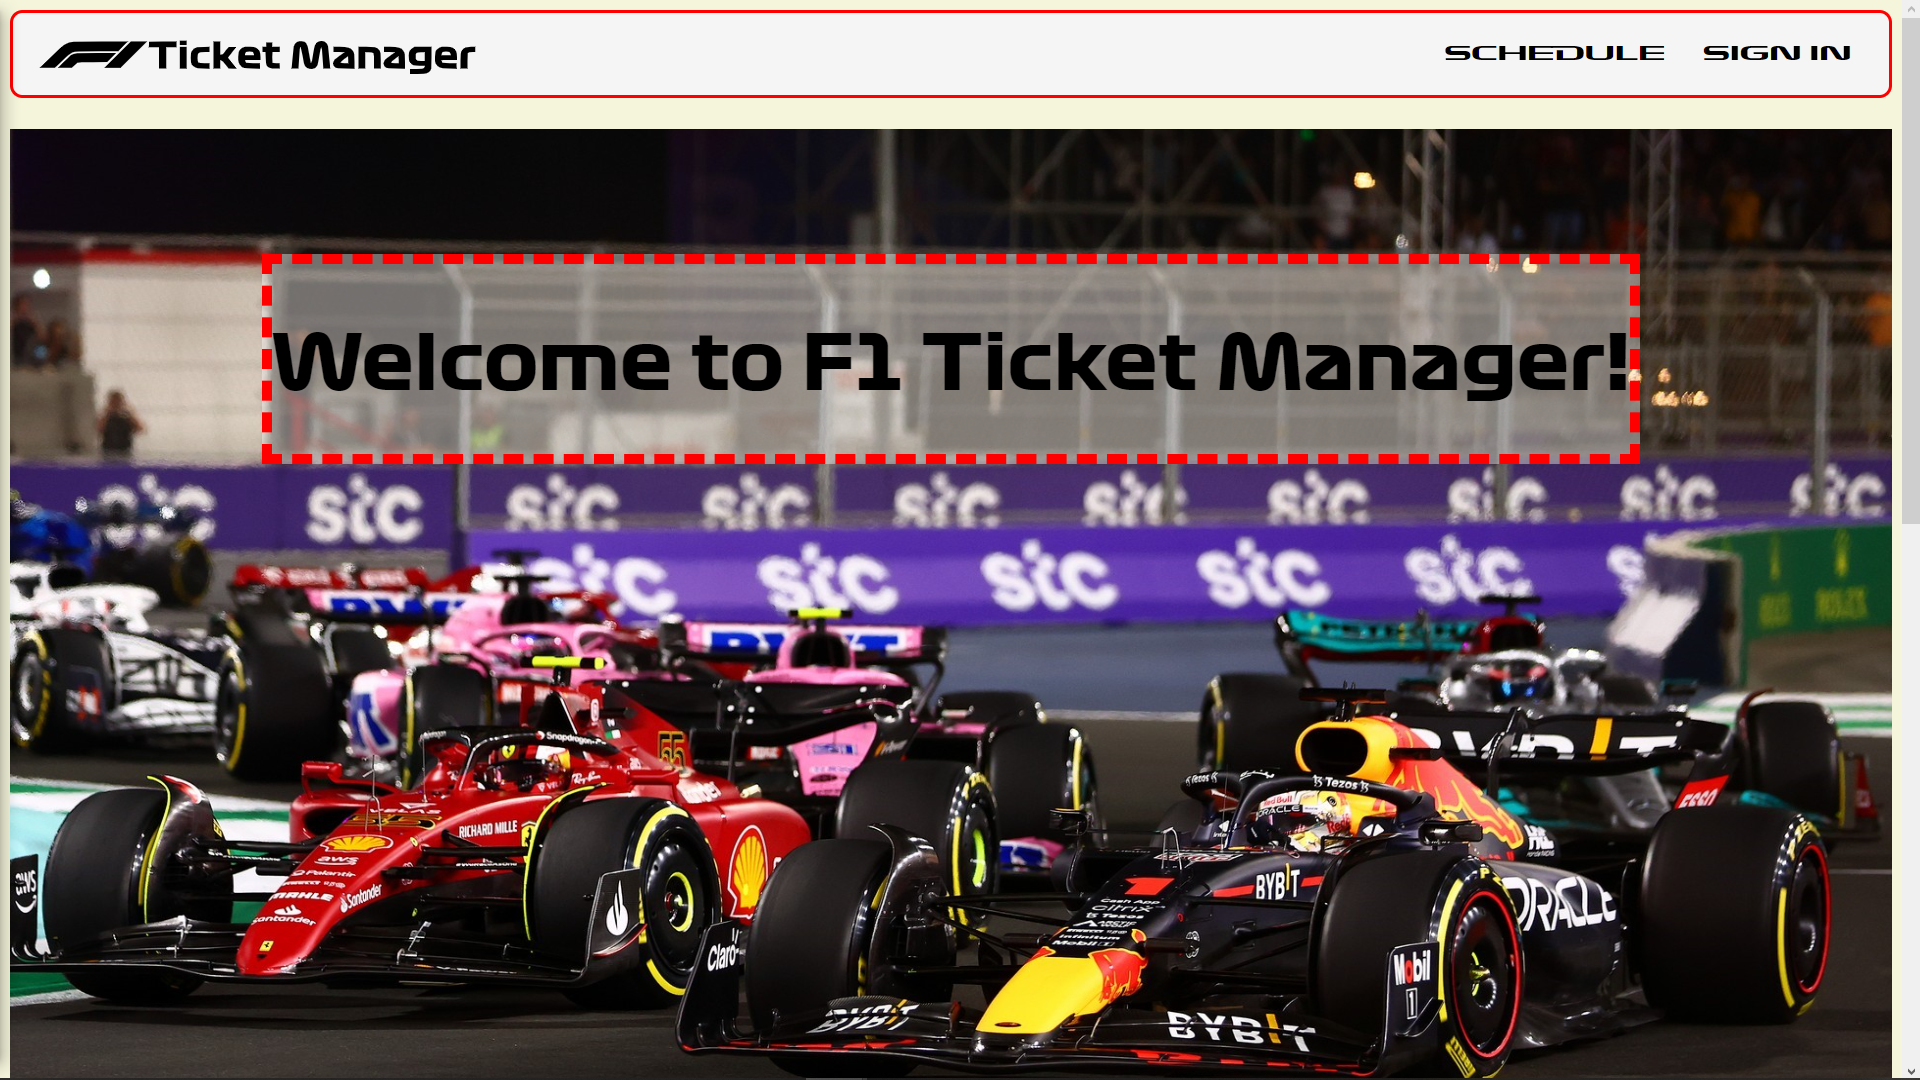
\includegraphics[scale=0.2]{images/homepage}
	\caption{Kezdőoldal}
	\label{abra:homepage}
\end{figure}
\pagebreak

\subsection {Versenynaptár (Schedule)}

A \textbf{Versenynaptár} oldalon lehet böngészni a 2022-es év versenyeinek listáját a megrendezési sorrendben. Az első kártya, ami megjelenik az oldalon az a következő verseny, amely automatikusan kerül ki az aktuális dátum alapján. Teszt jelleggel van egy dátum kiválasztó gomb is, hogy ki lehessen próbálni, hogy egy adott dátumhoz melyik verseny lesz a legközelebb. Erre a kártyára kattintva meg lehet tekinteni a részleteket. Minden kártyán látszanak a legfontosabb információk az adott versenyről, mint a pálya neve, a rendező ország neve, az intervallum, amikor az esemény zajlani fog és a pályarajz (\ref{abra:schedule}).

\begin{figure}[!h]
	\centering
	\begin{tabular}{cc}
	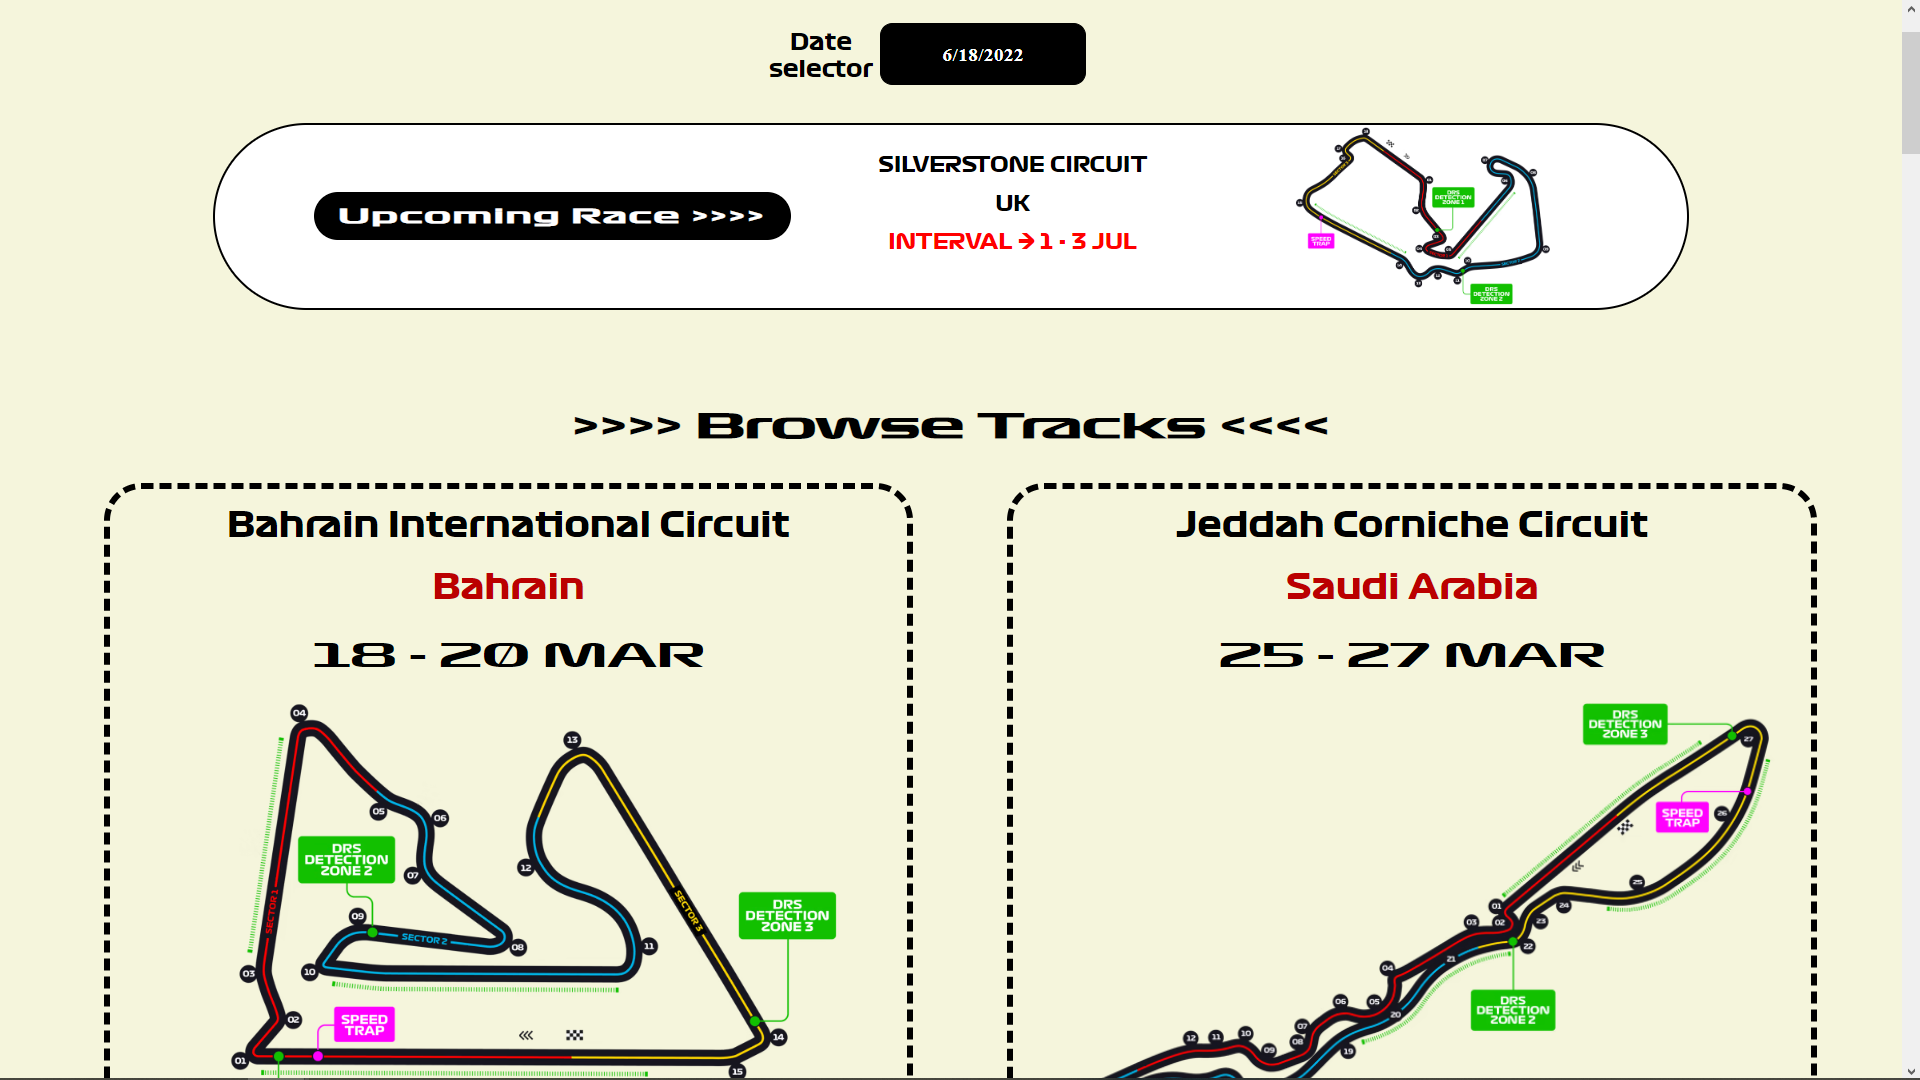
\includegraphics[scale=0.15]{images/schedule1} &
	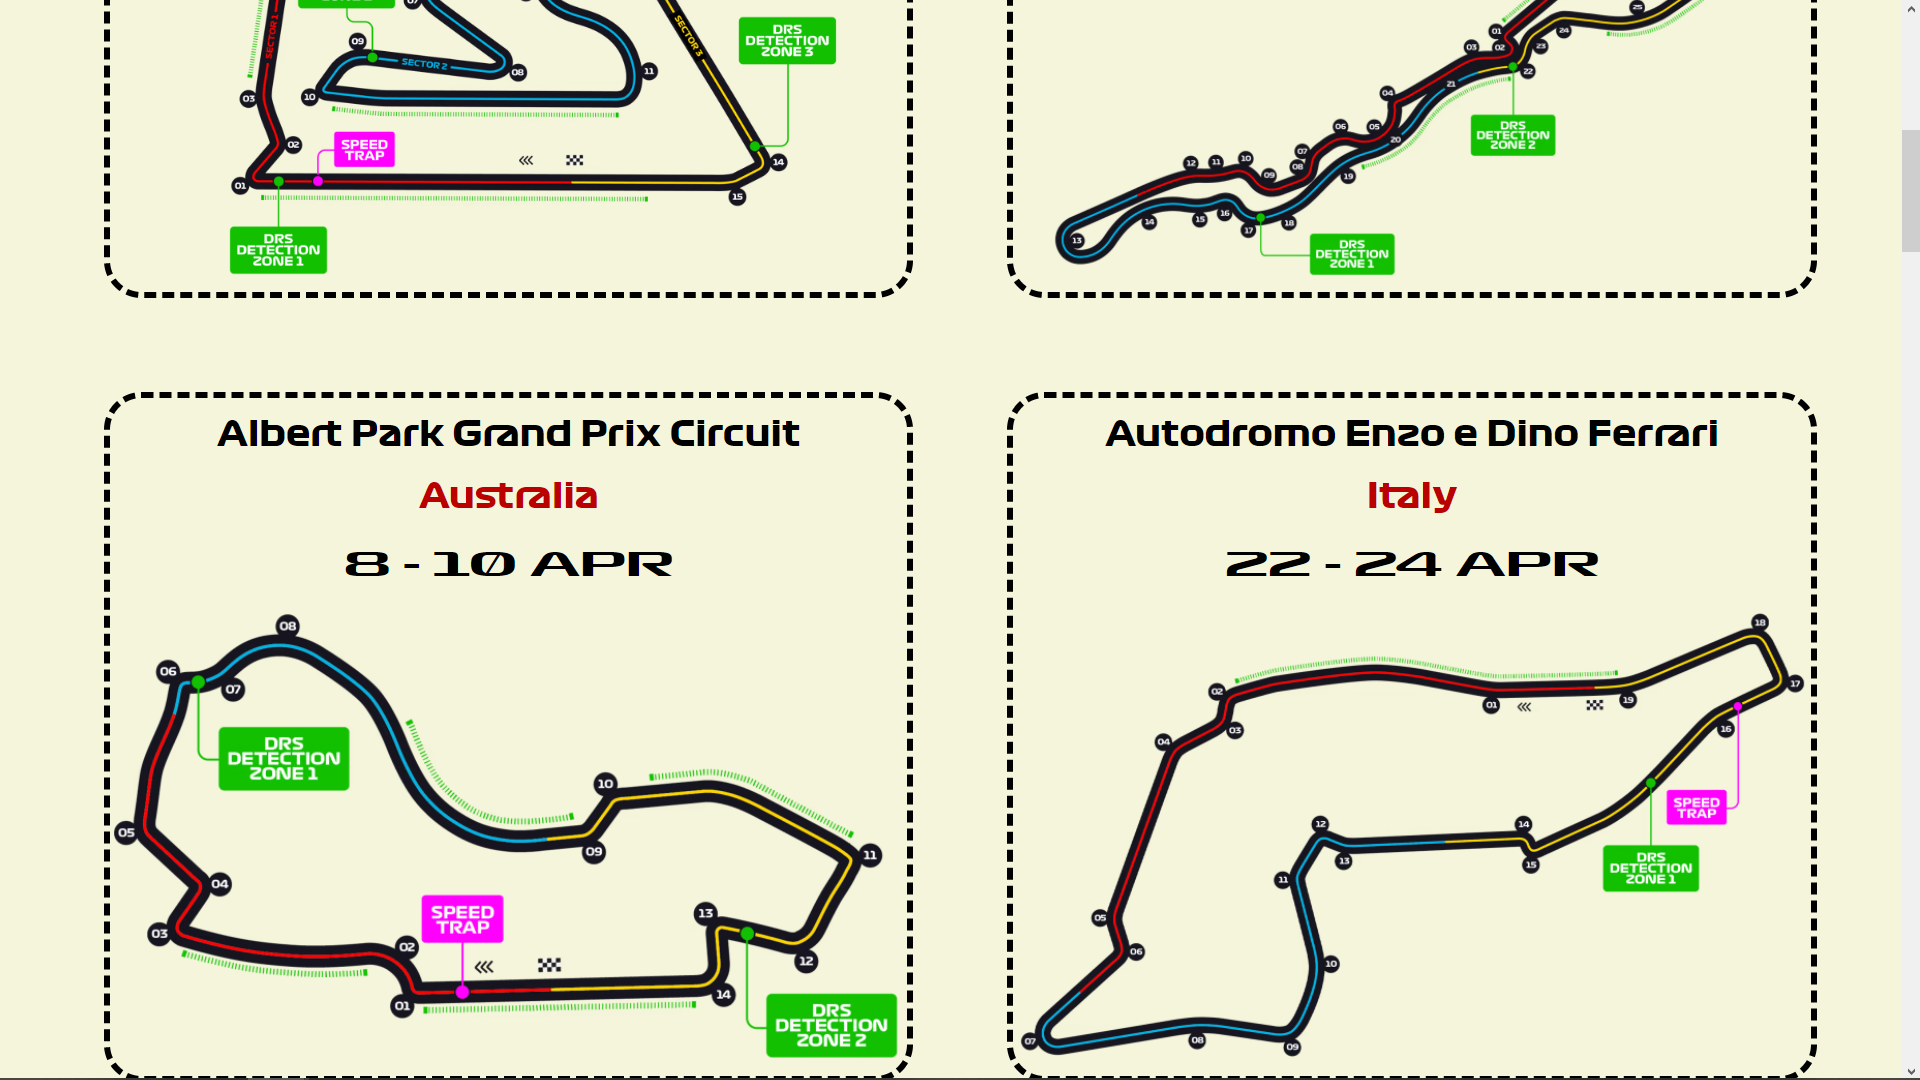
\includegraphics[scale=0.15]{images/schedule2} \\
	A versenynaptár & Görgetéssel látható az összes pálya
	\end{tabular}
	\caption{Versenynaptár}
	\label{abra:schedule}
\end{figure}

Ha átvisszük az egeret a kártya fölott, akkor megjelenik egy gomb \textbf{Browse tickets} szöveggel, amelyre kattintva megtekinthetőek a versenyhez tartozó jegy típusok és azok információi (\ref{abra:ticketsUA}). Ha nincs bejelentkezve a felhasználó, akkor az \textbf{Add to cart} gomb szürkén jelenik meg, vagyis nem lehet a kosárba tenni, viszont ha rákattint a felhasználó, akkor a rendszer jelezni fogja egy \textbf{alert} (figyelmeztetés) ablakban, hogy autentikáció szükséges, ha ezt a funkciót szeretné használni.

\begin{figure}[!h]
	\centering
	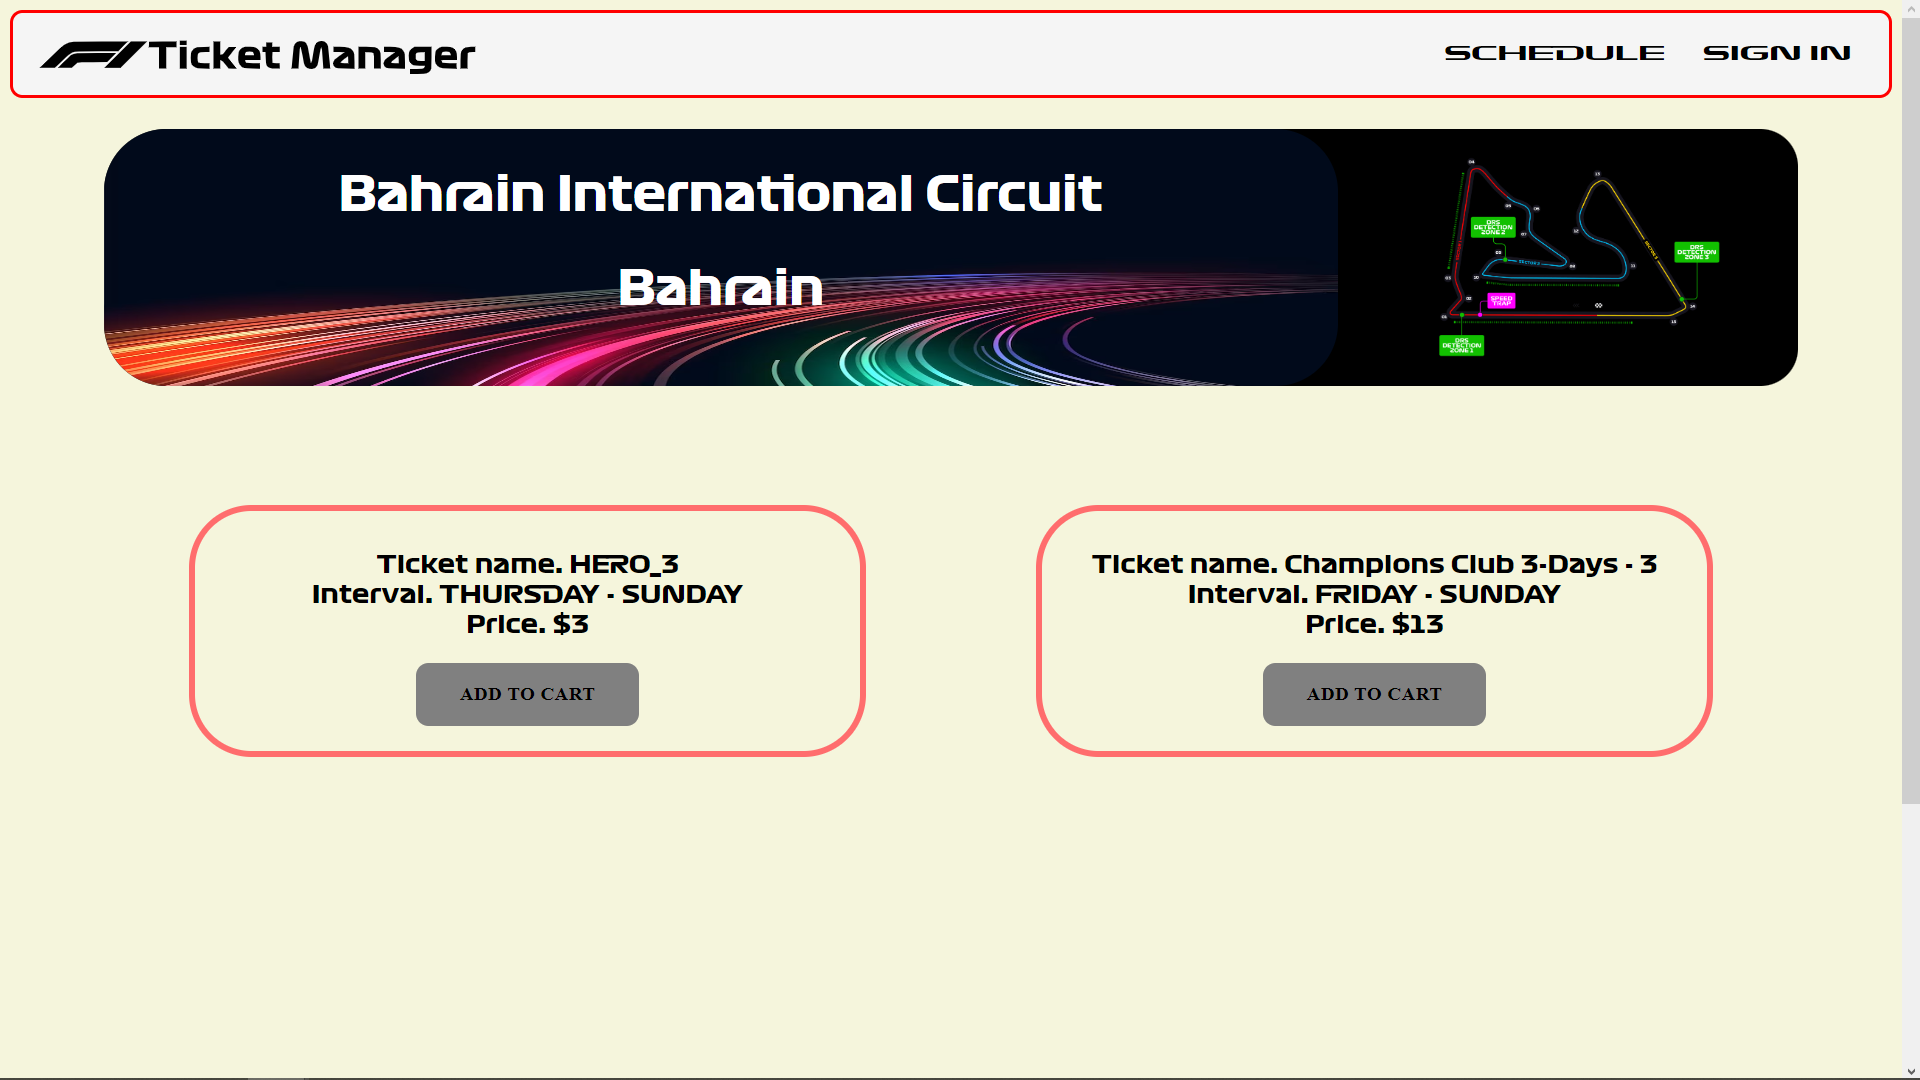
\includegraphics[scale=0.2]{images/tickets}
	\caption{Jegy típusok be nem jelentkezett felhasználóval}
	\label{abra:ticketsUA}
\end{figure}

Abban az esetben, ha a felhasználó be van jelentkezve, lehetőség van a jegyet a kosárba helyezni. Egy továbbfejlesztési lehetőség, hogy visszajelzést tudjon adni az adott jegyről, élményekről (\ref{abra:ticketsAuth}). A jegyek mennyiségét a \textbf{Checkout} oldalon van lehetősége módosítani a felhasználónak. A rendszer ezen része egy továbbfejlesztési terület, hogy adott esetben ellenőrizve legyen, hogy tényleg csak az tudjon visszajelzést adni, akkor vásárolt az adott jegyből. 

\begin{figure}[!h]
	\centering
	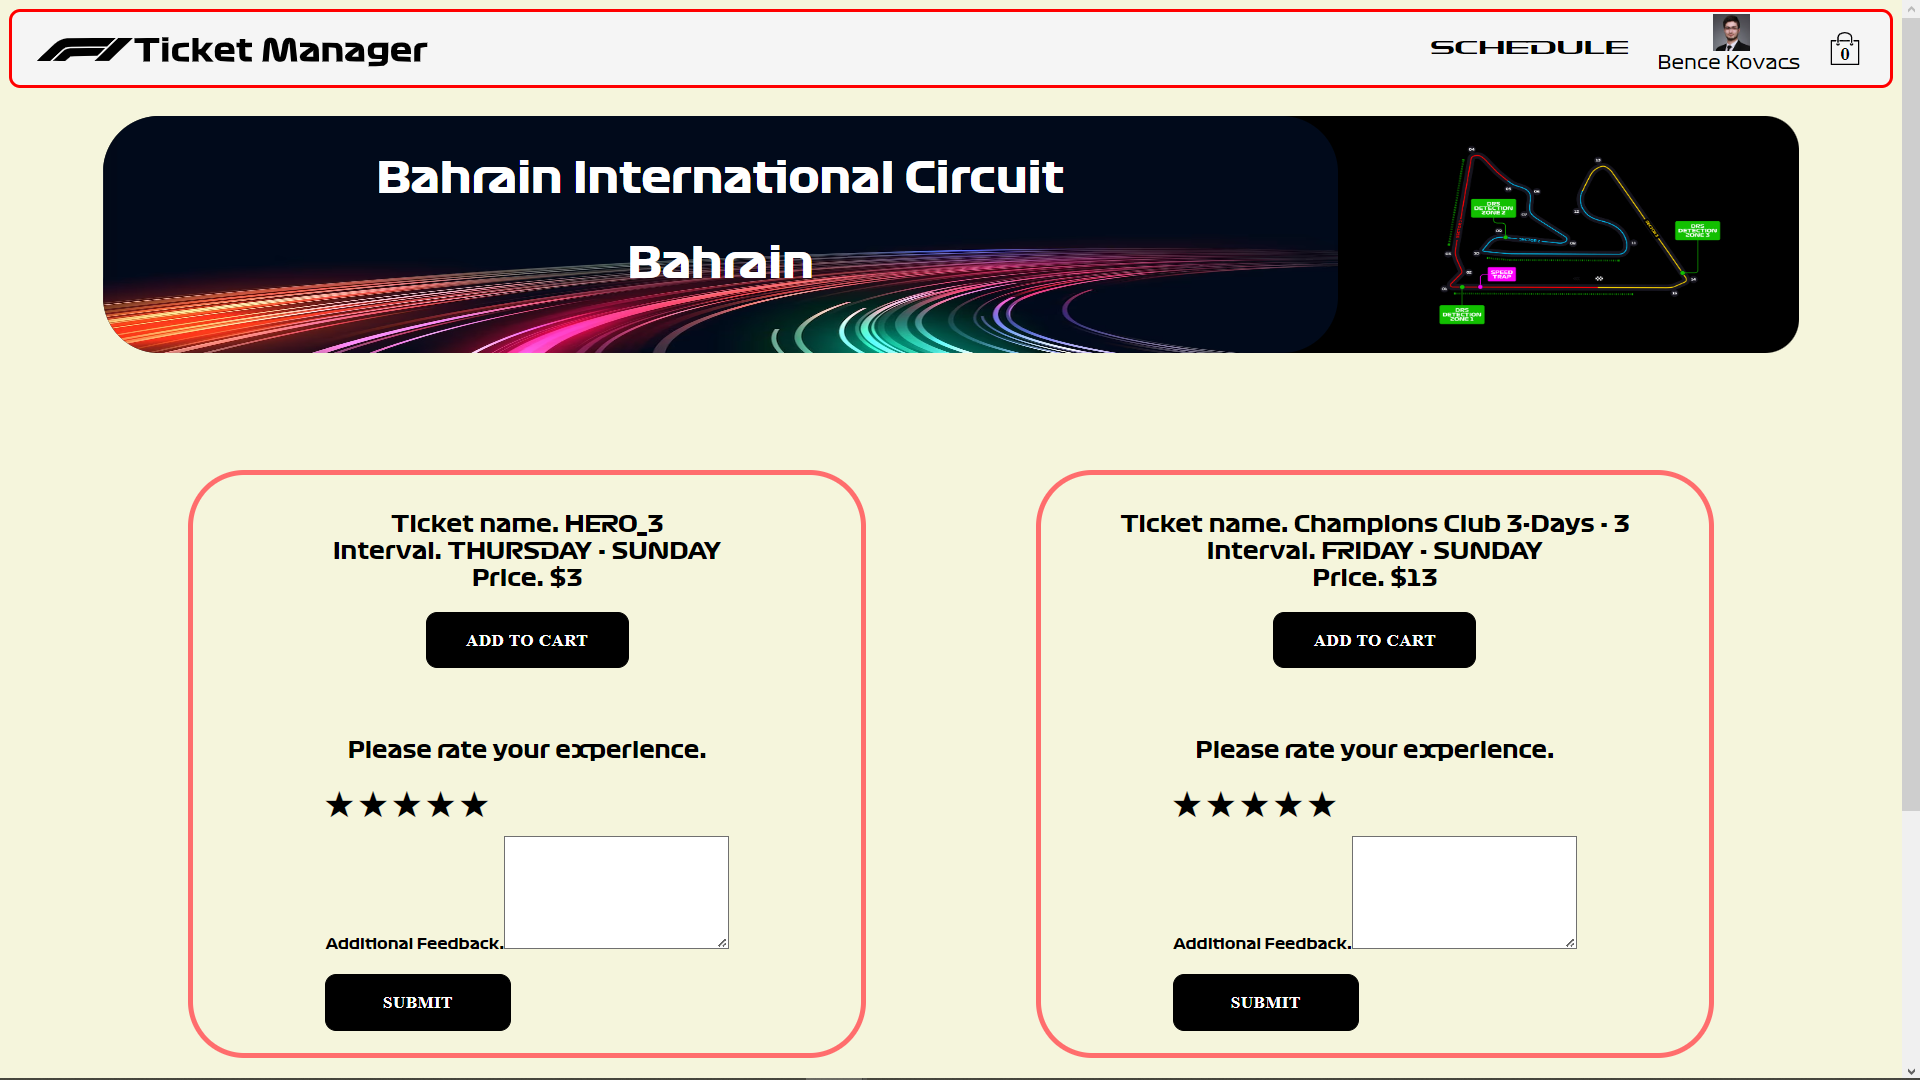
\includegraphics[scale=0.2]{images/ticketsAuth}
	\caption{Jegy típusok bejelentkezett felhasználóval}
	\label{abra:ticketsAuth}
\end{figure}

\subsection {Bejelentkezés és regisztráció (Sign in and up)}

A bejelentkezési felületen egyben lett feltüntetve a bejelentkezés és regisztráció két külön kártyán. Az email címmel vagy közösségi fiókkal való autentikáción kívül lehetőség van elfelejtett jelszó esetén új megadása. Ennek érdekében a felhasználó megadja az email címét és kapni fog egy levelet, amely tartalmaz egy linket az új jelszó megadásához (\ref{abra:signInUp}).

\begin{figure}[!h]
	\centering
	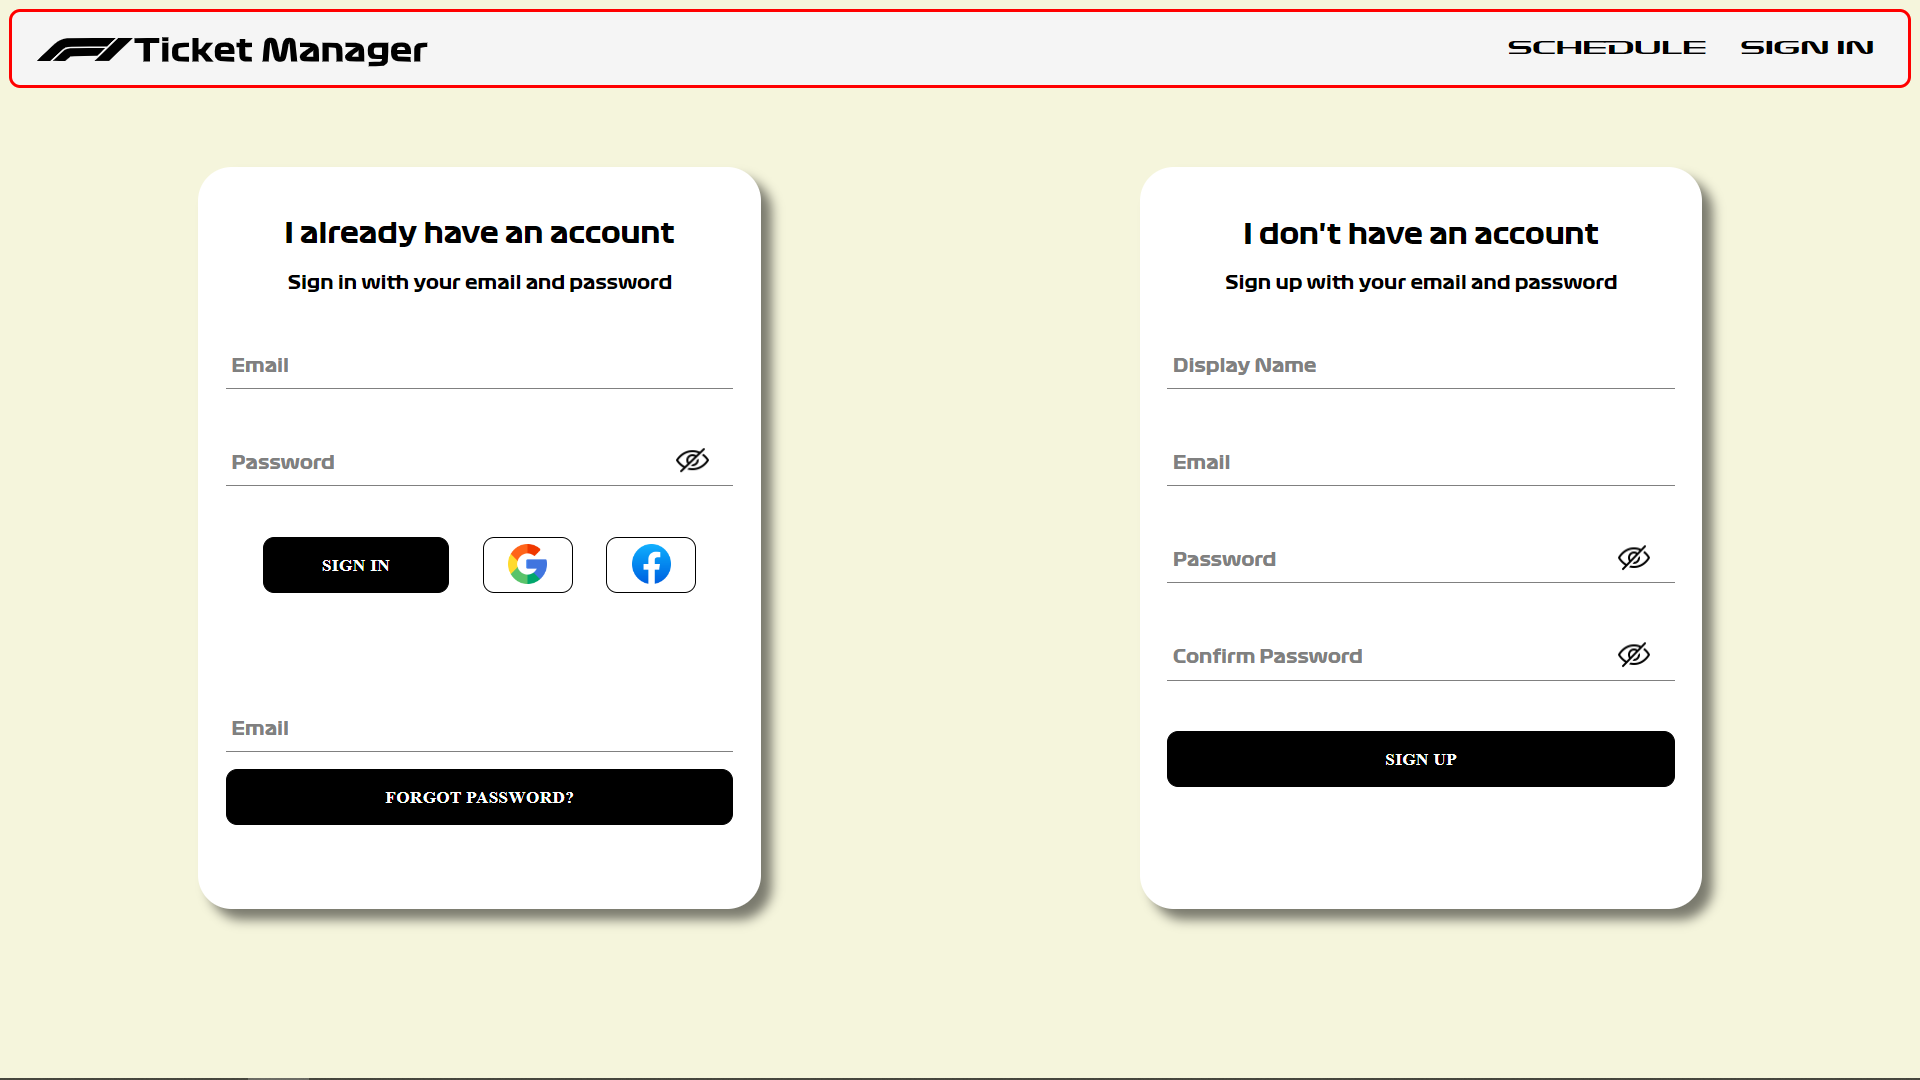
\includegraphics[scale=0.2]{images/signInUp}
	\caption{Autentikáció}
	\label{abra:signInUp}
\end{figure}

Továbbá lehetőség van a felületre való regisztrációra is a jobb oldali kártyán. Ennek a folyamatnak a bemutatására készítettem egy szekvencia diagramot a \textbf{SequenceDiagram.org} online szerkesztő segítségével \cite{Seq}.

\begin{figure}[!h]
	\centering
	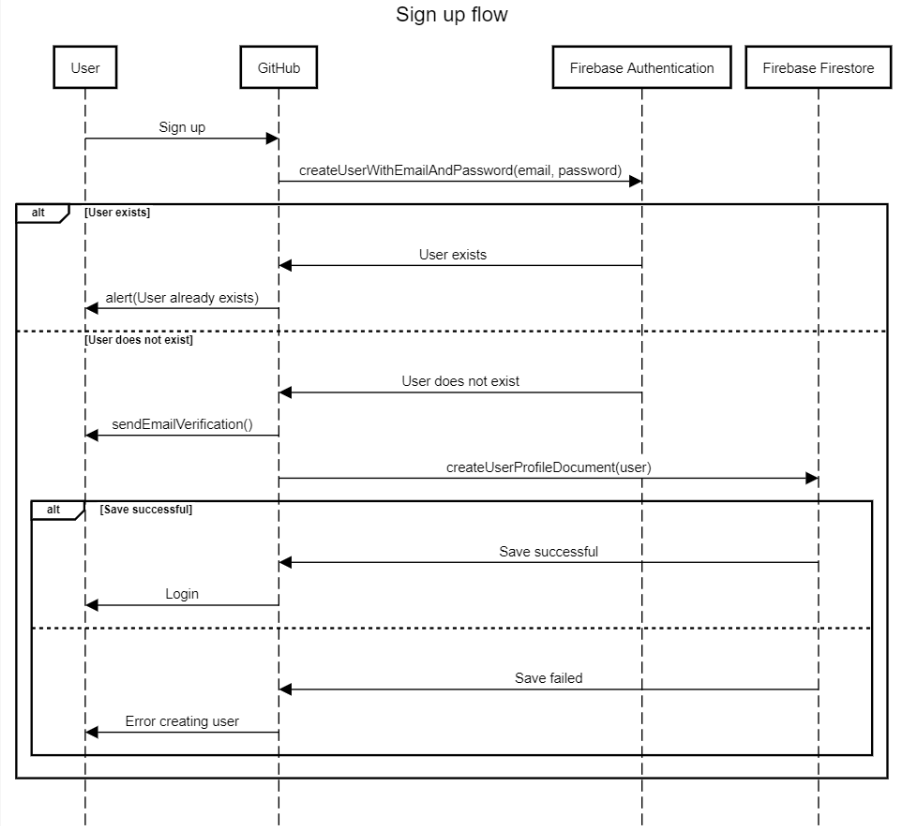
\includegraphics[scale=0.5]{images/signUpFlow}
	\caption{Szekvencia diagram - Regisztráció}
	\label{abra:signUpFlow}
\end{figure}
\pagebreak

A regisztráció folyamatát a felhasználó indítja el a kötelező mezők kitöltésével. A \textit{Firebase} szerver első sorban ellenőrzi, hogy az adott email címmel már létezik-e felhasználó és amennyiben igen, a megfelelő üzenetet jeleníti meg az oldal. Ellenkező esetben létrehozza a rendszerben a felhasználót, elmenti a megadott adatokat egyéb meta adatokkal kiegészítve, mint a létrehozás dátuma. A mentés után a rendszer automatikusan be is jelentkezteti a felhasználót (\ref{abra:signUpFlow}).

\subsection {Profil (Profile)}

A \textbf{Profil} oldal elérése csak a bejelentkezett felhasználóval lehetséges (\ref{abra:profile}). Ezen az oldalon lehetséges a profilkép és a megjelenített név módosítása az \textbf{Edit profile} gombra kattintva.

\begin{figure}[!h]
	\centering
	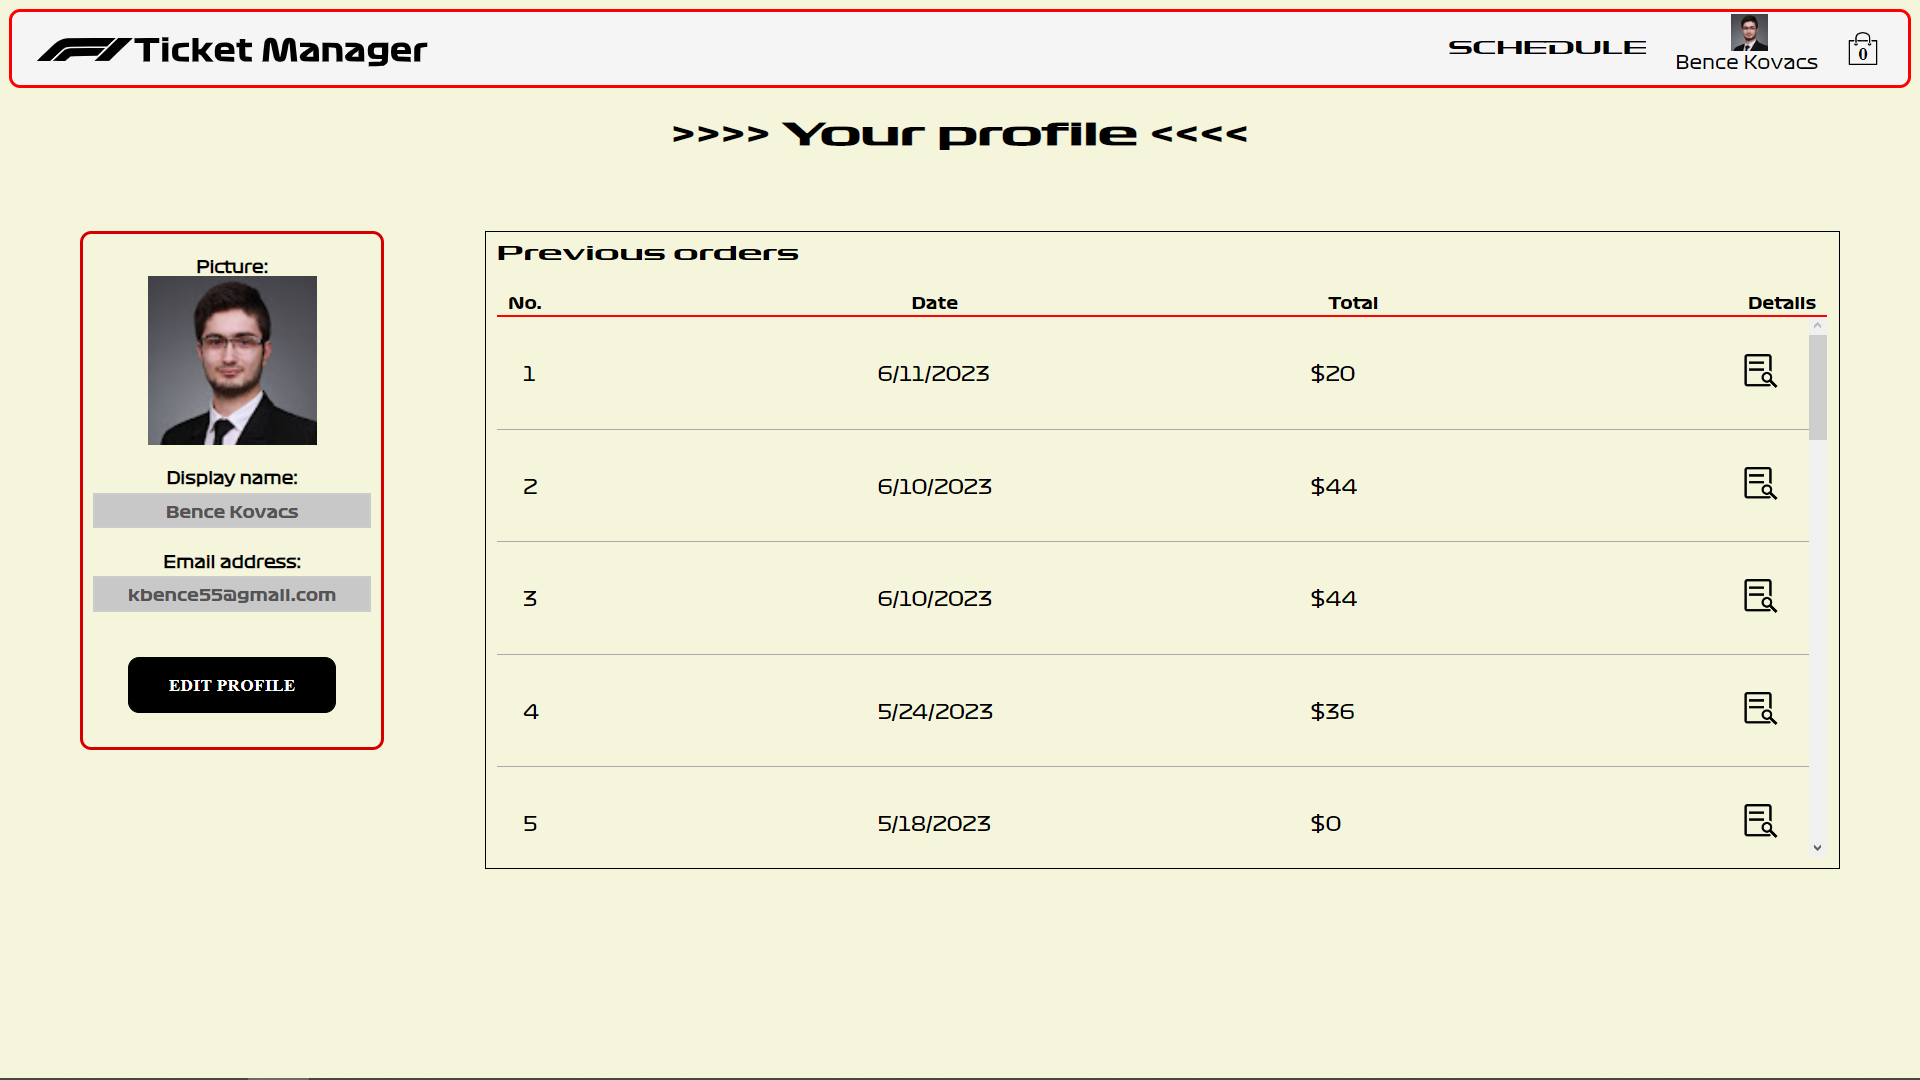
\includegraphics[scale=0.2]{images/profile}
	\caption{Saját profil oldal}
	\label{abra:profile}
\end{figure}

Az oldal jobb részén láthatóak a \textbf{rendelési előzmények}. Ezek görgetéssel böngészhetőek és a jobb szélén levő ikonra kattintva tekinthetőek meg a vásárlás részletei (\ref{abra:previousOrders}).

\begin{figure}[!h]
	\centering
	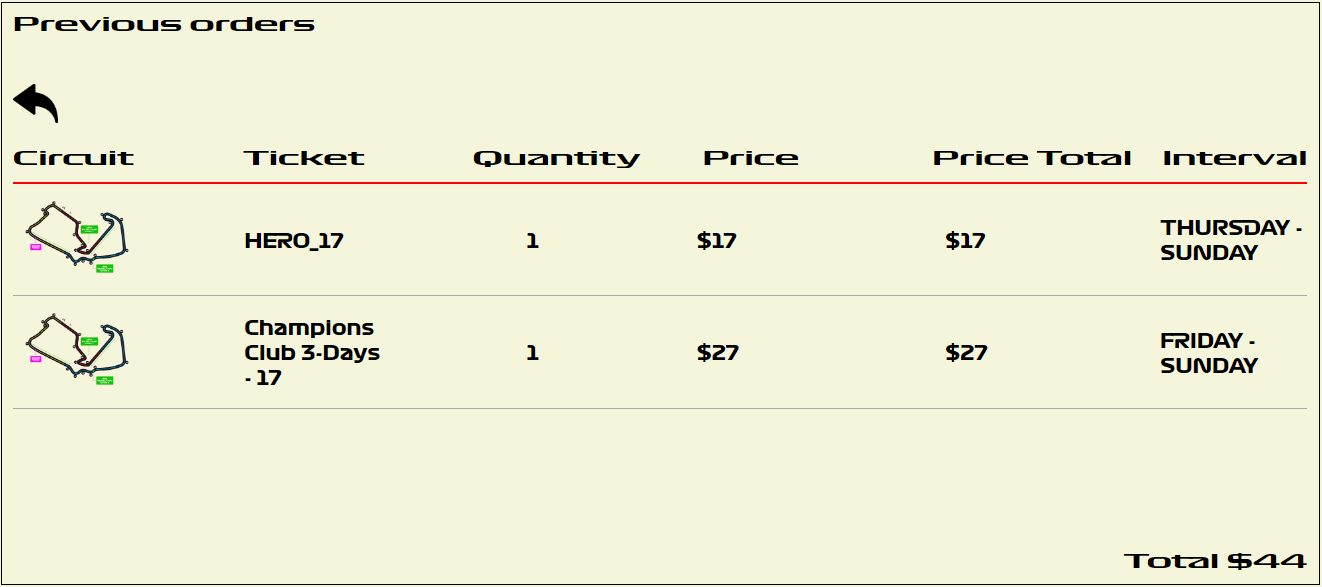
\includegraphics[scale=0.3]{images/previousOrders}
	\caption{Rendelés részletei}
	\label{abra:previousOrders}
\end{figure}

Amennyiben elvisszük valamely elem fölött az egeret megjelenik egy \textbf{More details} gomb, amelyre kattintva megtekinthető a jegy egyedi azonosítója (\ref{abra:moreDetails}). Ez a funkcionalitás azért fontos, mivel megtörténhet, hogy a felhasználó elveszíti vagy nem kapja meg a QR kódot emailben, ami ezt az azonosítót tartalmazza. Ha ez bekövetkezne, akkor innen is lehetőség van kimásolni és a megszokott módon azonosítani a PIN kóddal.

Ezen a felugró ablakon továbbá lehetősége van a felhasználónak egy új PIN kódot megadni, ha az aktuálist elfelejtette vagy úgy érzi, hogy valaki megszerezhette. Ezután egy újabb felugró ablakban lehetséges a PIN kód megváltoztatása. 

\begin{figure}[!h]
	\centering
	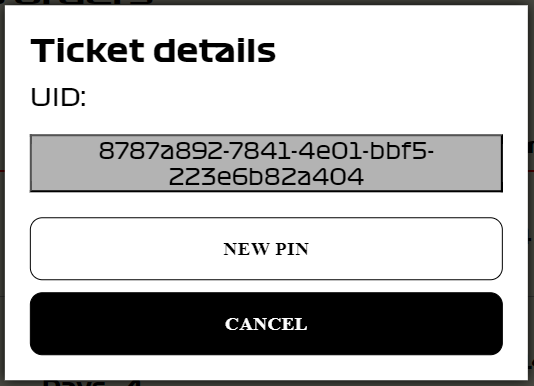
\includegraphics[scale=0.4]{images/moreDetails}
	\caption{Jegy részletei}
	\label{abra:moreDetails}
\end{figure}

A PIN kód megadásánál kötelezően egy 6 számjegyű számot kell megadni (\ref{abra:pinPopup}). Ezt manuálisan is be lehet írni vagy a \textit{pálca} ikonra kattintva generálódik egy véletlenszerű szám. A \textbf{Submit} gombra kattintva frissítheti a felhasználó a jegyhez tartozó kódot, ami teljes mértékben felülírja az előzőt, ezért nagyon figyelmes kell lenni a megadásakor, de erre a pirossal írt szöveg is figyelmezteti a vásárlót.

\begin{figure}[!h]
	\centering
	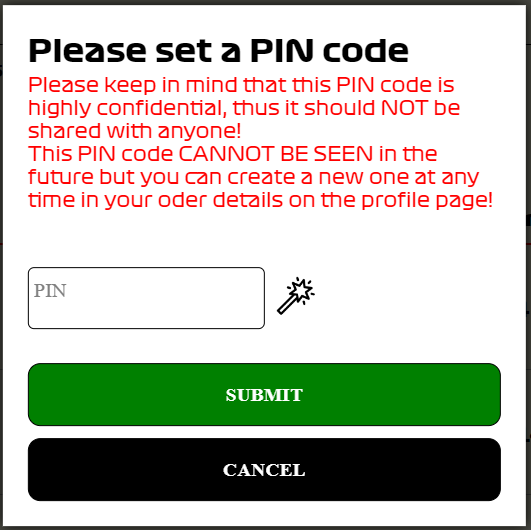
\includegraphics[scale=0.4]{images/pinPopup}
	\caption{PIN kód megadása}
	\label{abra:pinPopup}
\end{figure}
\pagebreak

\subsection {Rendelés (Checkout)}

A \textbf{Rendelés} oldalon van lehetősége a felhasználónak véglegesíteni a vásárlást (\ref{abra:checkout}). Itt is láthatóak a kosárba helyezett jegyek információi és csak itt módosíthatóak az egyes jegyek mennyisége vagy a kosárból való törlése. A \textbf{Pay Now} gombra kattintva a felhasználó meg tudja adni a számlázási adatokat majd a kártyaadatokat a vásárlás véglegesítéséhez. Ezt a \textbf{Stripe} szolgáltatás segítségével valósítottam meg. Sikeres vásárlás esetén a felhasználónak küld a rendszer egy emailt, amiben megkapja a QR kódokat. Egy kód tartalmazza a rendelés egyedi azonosítóját kombinálva a felhasználó egyedi azonosítójával. Az emailek küldésére a \textbf{Brevo} szolgáltatót vettem igénybe \cite{Brevo}.

\begin{figure}[!h]
	\centering
	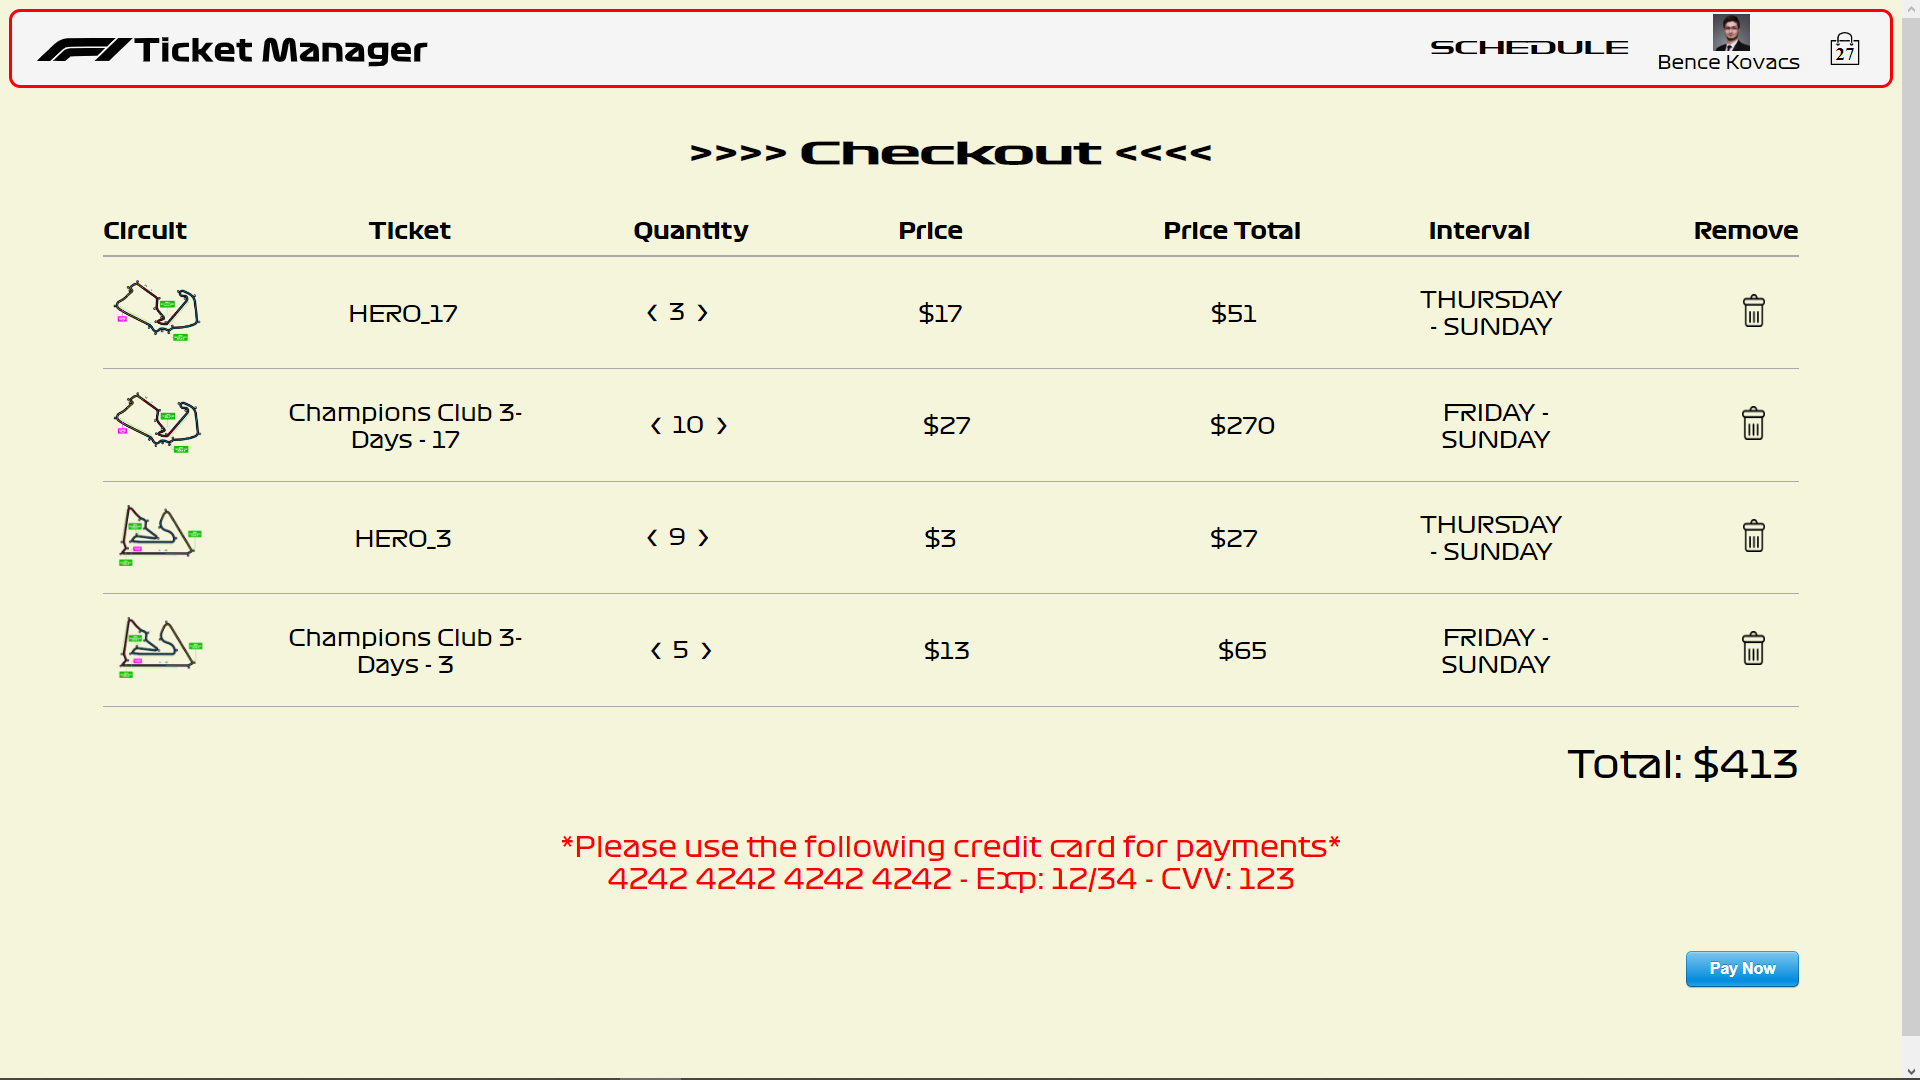
\includegraphics[scale=0.2]{images/checkout}
	\caption{Rendelés véglegesítése}
	\label{abra:checkout}
\end{figure}

A rendelés leadása után az adatok eltárolására használt titkosítás elvégzésére több megoldást is kipróbáltam, amelyek közül az egyik az \ref{code:encryption} kódrészlet, amely az AES algoritmus egyik használati módja JavaScript programozási nyelven a CryptoJS könyvtárcsomag segítségével.

A kód első lépése a \textit{salt (só)} generálása, ami egy 128/8 bájt szekvencia, amely segítségével meghatározásra kerül majd a key (kulcs). A \textit{CryptoJS.lib.WordArray.random(128 / 8)} kódsor a \textbf{CryptoJS} könyvtárban található \textit{random()} függvény hívásával egy véletlenszerű 128-bites szekvenciát generál, majd beilleszti az adatokat a WordArray osztályba.

A következő lépésben a kulcs előállítása történik meg a \textit{secretPass (jelszó)} és a só használatával a kulcsderiváló függvény segítségével. A kulcs előállítása a \textit{CryptoJS.PBKDF2()} függvénnyel történik, amely egy kulcstervező függvény. Az első paraméter a titkosításhoz használt jelszó, a második argumentum a só, a harmadik pedig a kulcs hosszát és az iterációk számát határozza meg. Ennél az algoritmusnál nagyon fontos odafigyelni, hogy a jelszó szigorúan titkos információ, vagyis ezt biztonságosan ajánlott eltárolni szerver oldalon. A többi paraméter publikus, mert önmagukban nem elegendőek a titkosított szöveg visszafejtéséhez.

Az inicializáló \textit{vektor (iv)} generálása következik. Az IV egy véletlenszerű bájt szekvencia, amelynek hossza megegyezik a blokk méretével (128 bit), és a titkosítás során használják, hogy azonos adatok esetén is véletlenszerű kimenetet generáljon.

Az adat titkosítása a \textit{CryptoJS.AES.encrypt()} függvénnyel történik. Az adatot először JSON formátumba alakítjuk, majd az AES algoritmust a kulcs, az IV és további paraméterek (mód, padding és tag) megadásával alkalmazzuk. A \textit{mode} a blokktitkosítási mód (BCM) kiválasztására szolgál, ezek között található a ECB, CBC, OFB vagy CFB. A mi esetünkben a CBC (Cipher Block Chaining) mód van használva.

\begin{lstlisting}[caption={Titkosítás példakód.}, captionpos=b, language = JavaScript, label={code:encryption}]
export const encryptData = text => {
  const salt = CryptoJS.lib.WordArray.random(128 / 8);
  const key = CryptoJS.PBKDF2(secretPass, salt, {
    keySize: 256 / 32,
    iterations: 1000,
  });
  const iv = CryptoJS.lib.WordArray.random(128 / 8);

  const encrypted = CryptoJS.AES.encrypt(JSON.stringify(text), key, {
    iv: iv,
    mode: CryptoJS.mode.CBC,
    padding: CryptoJS.pad.Pkcs7,
    tag: true,
  });

  const data = {
    ciphertext: encrypted.ciphertext.toString(CryptoJS.enc.Base64),
    iv: iv.toString(CryptoJS.enc.Base64),
    salt: salt.toString(CryptoJS.enc.Base64),
    tag: true,
  };
  return JSON.stringify(data);
};
\end{lstlisting}

A \textit{padding} a blokkok kitöltési módját határozza meg, itt a \textbf{Pkcs7} (Public Key Cryptography Standards 7-es szabványa) van használva. A Pkcs7 padding szabvány szerint, ha az üzenet hossza nem egész blokk méretű, akkor azt szükséges kiegészíteni. Minden hiányzó bájt felveszi a hiányzó bájtok számának megfelelő értéket. Ha például az utolsó blokkban 3 hiányzó bájt van, akkor a blokk utolsó bájtjai a 0x03 értéket veszi fel.

Az \textit{iv} az inicializáló vektort tartalmazza, amit korábban generáltunk. A textit{tag} beállítása igazra van állítva, hogy az üzenet hitelesítése (integritásának ellenőrzése) is megtörténjen a titkosítás során. A tag az üzenet elejére kerül beillesztésre a titkosítás során, és végül az eredeti üzenet végén kerül ellenőrzésre a helyessége.

Az utolsó lépés a \textit{titkosított adat (ciphertext)}, az IV, a só és az üzenet hitelesítésének értéke (tag) összekapcsolása és JSON formátumba rendezése és visszatérítése.

Az alábbi példakód a visszafejtést valósítja meg (\ref{code:decryption}):

\begin{lstlisting}[caption={Visszafejtés példakód.}, captionpos=b, language = JavaScript, label={code:decryption}]
export const decryptData = text => {
const json = JSON.parse(text);
const salt = CryptoJS.enc.Base64.parse(json.salt);
const iv = CryptoJS.enc.Base64.parse(json.iv);
const tag = json.tag;
const ciphertext = CryptoJS.enc.Base64.parse(json.ciphertext);

const key = CryptoJS.PBKDF2(secretPass, salt, {
	keySize: 256 / 32,
    	iterations: 1000,
});

const decrypted = CryptoJS.AES.decrypt(
  	{ ciphertext: ciphertext, salt: salt, iv: iv, tag: tag },
    	key,
    	{
     	iv: iv,
      	mode: CryptoJS.mode.CBC,
      	padding: CryptoJS.pad.Pkcs7,
      	tag: true,
    }
  );
  return JSON.parse(decrypted.toString(CryptoJS.enc.Utf8));
};
\end{lstlisting}

A \textbf{decrypt} függvény az \textbf{encrypt} függvénnyel ellentétes sorrendben dolgozza fel az adatokat. A paraméterként kapott titkosított szövegből JSON objektumot állít elő. Ezután ebből az objektumból megkapja a só és az iv Base64 formátumból az értékeket. A kulcs előállítása a \textit{PBKDF2} függvénnyel történik a jelszó és a só segítségével. A titkosított adat, az iv, a só és a hitelesítési tag felhasználásával sikeresen vissza tudjuk fejteni az eredeti üzenetet.

A másik opció a \textbf{CryptoJS} csomag mellett a \textbf{node-rsa} könyvtárcsomag segítségével megvalósított titkosítás és RSA kulcscsere volt \textbf{NodeJS} keretrendszerben. A \ref{code:rsaEncrypt} kódrészletben az adat titkosítása látható a RSA publikus kulcs segítségével (\ref{code:rsaGenrerate} kódrészlet), amelyet minden rendelés során a rendszer generál a privát kulcs mellett. A titkosítás során szükség van a \textit{publicKey}-re, amely a generálás során elmentődik az adatbázisba és ezt lekéri a rendszer. A publicKey segítségével titkosítom az \textit{AES} kulcsot, amellyel titkosítom az eredeti szöveget. A végeredmény egy \textbf{encryptedData} és egy \textbf{encryptedKey} lesz, amelyek hasonlóan bekerülnek az adatbázisba az összesített rendelések közé, az \textbf{orders} dokumentumba.

\begin{lstlisting}[caption={RSA kulcscsere és titkosítás.}, captionpos=b, language = JavaScript, label={code:rsaEncrypt}]
const aesKey = CryptoJS.lib.WordArray.random(16).toString();
const encryptedData = CryptoJS.AES
	.encrypt(<unique code with PIN code>, aesKey).toString();

const rsaKey = new NodeRSA();
rsaKey.importKey(publicKey, "public");
const encryptedKey = rsaKey.encrypt(aesKey.toString(), "base64");
\end{lstlisting}

\begin{lstlisting}[caption={RSA kulcsok generálása.}, captionpos=b, language = JavaScript, label={code:rsaGenrerate}]
const key = new NodeRSA({ b: 2048 });
const publicKey = key.exportKey("public");
const privateKey = key.exportKey("private");
\end{lstlisting}

A \ref{code:rsaDecrypt} kódrészletben lekéri a rendszer a rendeléshez tartozó privát kulcsot, majd annak segítségével visszafejti a titkosított \textit{AES} kulcsot. Ezzel a kulccsal már vissza lehet fejteni a titkosított szöveget, ezáltal megkapni a az eredeti szöveget az egyedi azonosítóval és a PIN kóddal.

\begin{lstlisting}[caption={RSA visszafejtés.}, captionpos=b, language = JavaScript, label={code:rsaDecrypt}]
const rsaKey = new NodeRSA();
rsaKey.importKey(privateKey, "private");
const decryptedKey = rsaKey.decrypt(data?.encryptedKey, "utf8");

const decryptedData = CryptoJS.AES.decrypt(
	data?.encryptedData,
	decryptedKey
).toString(CryptoJS.enc.Utf8);
\end{lstlisting}

\pagebreak
\subsection {Beléptetés (Scan)}

A \textbf{Beléptetés} oldalon a rendszer \textit{Adminisztrátora(i)} tudják a jegyeket hitelesíteni a versenyhelyszíneken az erre a célra kihelyezett termináloknál (\ref{abra:scan}). A felhasználó a kamera elé helyezi a QR kódot \cite{RQR}, majd beírja a PIN kódot, amelyeket a rendszer rögzít és jelzi a hitelesítési folyamat eredményét.

\begin{figure}[!h]
	\centering
	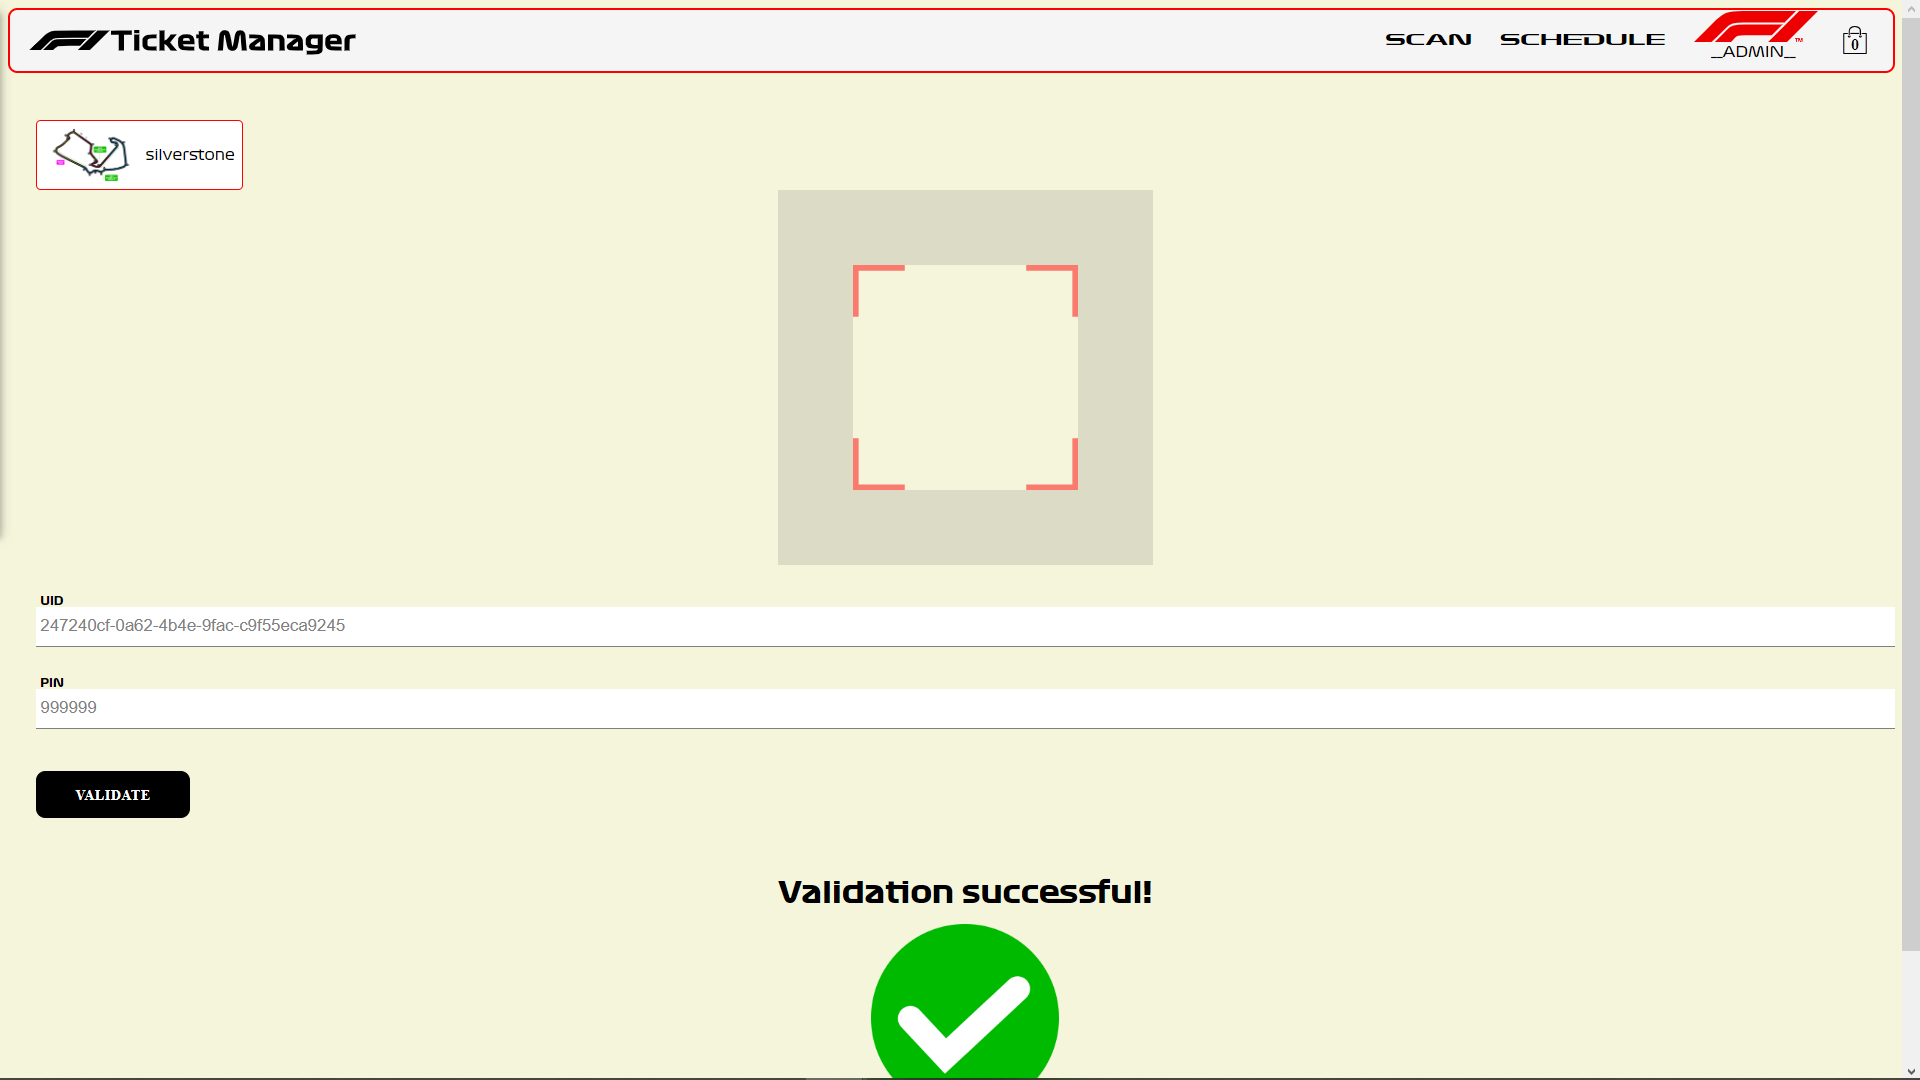
\includegraphics[scale=0.2]{images/scan}
	\caption{Jegyek hitelesítése}
	\label{abra:scan}
\end{figure}
	%----------------------------------------------------------------------------
\chapter{Szoftver}
%----------------------------------------------------------------------------


\begin{center}
	\begin{algorithm}[H]
		\KwIn{
			Integers $a \geq 0$ and $b \geq 0$}
		\KwOut{\textsc{Gcd} of $a$ and $b$} \While{$b \neq 0$}{
			$r \leftarrow a \bmod b$\;
			$a \leftarrow b$\;
			$b \leftarrow r$\;
		}
		\caption{Euclidean Algorithm}
	\end{algorithm}
\end{center}







\begin{algorithm}[H]
	\SetAlgoLined
	\KwData{this text}
	\KwResult{how to write algorithm with \LaTeX2e }
	initialization\;
	\While{not at end of this document}{
		read current\;
		\eIf{understand}{
			go to next section\;
			current section becomes this one\;
		}{
			go back to the beginning of current section\;
		}
	}
	\caption{How to write algorithms}
\end{algorithm}

\newpage
\begin{algorithm}[H]
	\DontPrintSemicolon
	\KwData{$G=(X,U)$ such that $G^{tc}$ is an order.}
	\KwResult{$G’=(X,V)$ with $V\subseteq U$ such that $G’^{tc}$ is an
		interval order.}
	\Begin{
		$V \longleftarrow U$\;
		$S \longleftarrow \emptyset$\;
		\For{$x\in X$}{
			$NbSuccInS(x) \longleftarrow 0$\;
			$NbPredInMin(x) \longleftarrow 0$\;
			$NbPredNotInMin(x) \longleftarrow |ImPred(x)|$\;
		}
		\For{$x \in X$}{
			\If{$NbPredInMin(x) = 0$ {\bf and} $NbPredNotInMin(x) = 0$}{
				$AppendToMin(x)$}
		}
		\nl\While{$S \neq \emptyset$}{\label{InRes1}
			\nlset{REM} remove $x$ from the list of $T$ of maximal index\;\label{InResR}
			\lnl{InRes2}\While{$|S \cap ImSucc(x)| \neq |S|$}{
				\For{$ y \in S-ImSucc(x)$}{
					\{ remove from $V$ all the arcs $zy$ : \}\;
					\For{$z \in ImPred(y) \cap Min$}{
						remove the arc $zy$ from $V$\;
						$NbSuccInS(z) \longleftarrow NbSuccInS(z) - 1$\;
						move $z$ in $T$ to the list preceding its present list\;
						\{i.e. If $z \in T[k]$, move $z$ from $T[k]$ to
						$T[k-1]$\}\;
					}
					$NbPredInMin(y) \longleftarrow 0$\;
					$NbPredNotInMin(y) \longleftarrow 0$\;
					$S \longleftarrow S - \{y\}$\;
					$AppendToMin(y)$\;
				}
			}
			$RemoveFromMin(x)$\;
		}
	}
	\caption{IntervalRestriction\label{IR}}
\end{algorithm}
\newpage
\section {A szoftver bemutatása}

Az általam írt szoftver egy \textbf{Java nyelv}en, \textbf{NetBeans IDE 8.0.1} fejlesztői környezetben írt asztali alkalmazás, amelynek fő funkcionalitása a kezdetiérték-probléma típusú differenciálegyenletek numerikus megoldása és ezen megoldások grafikus felületen való ábrázolása. A fő funkcionalitás mellett a szoftver tartalmaz még két kisebb funkcionalitást is, ezek közül az egyik a kétdimenziós függvényábrázolási lehetőség, a másik pedig a háromdimenziós függvények megjelenítésének lehetősége.

Az szoftver a differenciálegyenletek megoldásához a \ref{fejezet3}. fejezetben leírt numerikus eljárásokat alkalmazza.

A grafikus felhasználói felület megalkotásához a \textbf{Swing} (Java) komponens készletet használtam. A Swing használatával célom az volt, hogy egy felhasználóbarát és könnyen kezelhető felületet hozzak létre, amelyen a felhasználó könnyedén eligazodhat. Továbbá e komponenskészlet használata mellett szól az is, hogy a későbbiekben bemutatásra kerülő könyvtárak, melyek az ábrázolás megvalósítására használtam szintén Swing komponensekkel vannak megvalósítva.

Felhasználói felület, valamint a három funkcionalitás bemutatása képekben:

\begin{algorithm}[H]
	\Switch{order}{
		\uCase{bloody mary}{
			Add tomato juice\;
			Add vodka\;
			break\;
		}
		\uCase{hot whiskey}{
			Add whiskey\;
			Add hot water\;
			Add lemon and cloves\;
			Add sugar or honey to taste\; break\;
		}
		\Other{Serve wine\;}
	}
\caption{Switch haszn\'alata}
\end{algorithm}

\section {A szoftver megírásához használt könyvtárak}

	A szoftver elkészítésénél szükségem volt néhány előre megírt osztálykönyvtárra, amelyek megkönnyítették a munkámat. Ezekről tudni kell, hogy nyílt forráskódúak, tehát bárki számára elérhetőek az interneten, továbbá azt is, hogy ezek is Java nyelvben íródtak, hasonlóan, mint az általam írt alkalmazás. A továbbiakban szeretném bemutatni ezeket a könyvtárakat  és azt, hogy mire- és hogyan használtam fel őket.
	
	\begin{itemize}
		\item JMathPlot (\url{https://sites.google.com/site/mulabsltd/products/jmathplot}):
		\begin{itemize}
			\item Java könyvtár, amelyet interaktív megjelenítésre, ábrázolásra fejlesztettek
			\item gyors és könnyű utat biztosít tudományos adatok megjelenítésére Swing komponensek segítségével (nem használ openGL-t)
			\item az általa biztosított saját komponenseket úgy lehet használni, mint bármely más Swing komponenst
			\item a számomra legfontosabb tulajdonsága az, hogy két- és háromdimenziós ábrázolási lehetőséget biztosít, ezt használtam fel az alkalmazásomban
		\end{itemize}
		\item JMathArray (\url{https://sites.google.com/site/mulabsltd/products/jmatharray}):
		\begin{itemize}
			\item olyan Java könyvtár, amely alapvető matematikai, lineáris algebrai műveleteket biztosít számunkra 
			\item a könyvtár által biztosított statikus metódusok tömbökre alkalmazhatóak
			\item a szoftverben arra használtam, hogy egy megadott intervallum két végpontja között egy bizonyos lépésközzel haladva egy tömböt tudjak feltölteni (inkrementálás)
		\end{itemize}
		\item JEP (\url{http://www.cse.msu.edu/SENS/Software/jep-2.23/doc/website/}):
		\begin{itemize}
			\item szintén egy Java könyvtár, amelyet különböző elemzésekre és kiértékelésekre fejlesztettek
			\item segítségével egy szövegként (sztring-ként) megadott kifejezést könnyedén kiértékelhetünk, elvégezhetünk
			\item a szövegként megadott kifejezésből a háttérben egy kifejezésfát épít fel, majd a későbbiekben ennek a fának a segítségével dolgozik
			\item emellett sok általános matematikai függvény és konstans is bele van építve, amiket szintén könnyedén elérhetünk
			\item az általam fejlesztett szoftverben a függvények sztringként adhatók meg egy beviteli mezőn keresztül, a JEP könyvtárat ezen függvények „parszolására” használtam fel
%			\begin{figure}[h]
%				\centering
%				\includegraphics{figures/parszolas}
%				\caption{Egyszerű kifejezés elemzése, kiértékelése (Forrás: \url{http://www.singularsys.com/jep/doc/html/})}
%			\end{figure}
		\end{itemize}
	\end{itemize}

\pagebreak
\section {Diagramok}

\subsection{Use Case diagram}
%	\begin{figure}[!htb]
%		\centering
%		\includegraphics[width=1.0\textwidth]	{figures/diagramok/UsecaseDiagram.jpg}
%		\caption{Use Case diagram}
%	\end{figure}
\subsection{Osztálydiagram}
	A szoftver szerkezetileg két nagyobb részből (csomagból) áll, az egyik a felhasználói felület megalkotásához szükséges osztályokat tartalmazza, a másik pedig a differenciálegyenletek megoldására szolgáló osztályokat és a parszer osztályt, mely egy sztringként megadott függvény kiértékelésére szolgál.
	
	Az implementációnál a felhasználói felület elemeit tartalmazó csomagot „View”-nak, a numerikus módszereket és a parszert tartalmazó csomagot „Model”-nek neveztem, emellett a 6.7-es ábrán megjelenik egy harmadik csomag is, amely tartalmazza a „MainClass”-t és egyben a main() metódust is. Az alábbi két diagramon láthatjuk a felsorolt csomagokat és a bennük lévő osztályokat, illetve a köztük lévő kapcsolatokat.
	\pagebreak
	\begin{figure}
		\centering
		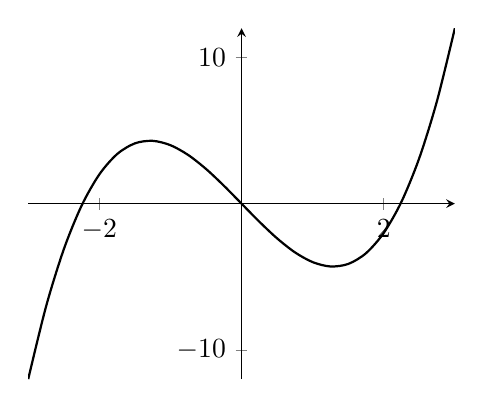
\begin{tikzpicture}
	\begin{axis} [axis lines=center]
		\addplot [domain=-3:3, smooth, thick] { x^3 - 5*x };
	\end{axis}
\end{tikzpicture}
\caption{Az $x^3-5x$ f\"uggv\'eny grafikus k\'epe PGFPLOT-al}
\end{figure}


\begin{figure}[h!]
	\centering
	\begin{tikzpicture}
		\begin{axis} [axis lines=center,xticklabels=\empty,yticklabels=\empty, xmin=-0.8,ymax=2.5,ytick style={draw=none}, xtick style={draw=none},tick,xlabel={$s$}]
			%N=6,p=3,p^*=6, p_*=5
			\addplot [domain=0:1, smooth, thick] { 1-2*x^(3) - 3*x^2  } node[midway,above right] {$\Psi$};
			\addplot[mark=*,color=red,] coordinates {(0.5,0)} node[midway,above right] {$\sigma^*$};
			\addplot[mark=*,color=red,] coordinates {(0,1)} node[midway,above left] {\scriptsize $\Psi(0)=\frac{1}{p2^{p-1}r_F^p}$};
		\end{axis}
	\end{tikzpicture}
	\caption{A $\Psi$ grafikus k\'epe}
\end{figure}
\pagebreak
\subsection{Szekvencia diagram}
 \pgfplotsset{compat=1.11}
\begin{figure}[h!]
	\centering
	\begin{tikzpicture}[
		% define a style for the dots
		dot/.style={
			draw=black,
			fill=red!90,
			circle,
			minimum size=3pt,
			inner sep=0pt,
			solid,
		},
		]
		\begin{axis}[
			xmin=-1,
			xmax=2,
			ymin=-0.5,
			ymax=3,
			axis lines=center,
			ticks=none,
			xlabel={$s$},
			xlabel style={below right},
			ylabel style={above left},
			% (moved common `addplot' options here)
			smooth,
			domain=0:2,
			samples=101,
			no markers,
			draw=black
			]
			\addplot [blue,thick] {(9*x^(5/2)-x^(11/2)-2*x^(9/2))/(1+x^(3/2)+x^(7/2)) } node [midway,above right,color=black] {$\Lambda(s)$};
			\addplot[color=red,] coordinates {(0,0)} node[midway,above left] {$\Lambda(0)$};
			% draw the dots (using the above defined style) and labels
			\draw[dashed,color=red] (0.95,0) node [dot,label=below:$s_{\rm max}$] {}-- (0.95,2.017873338) node [dot,label=above:$\Lambda(s_{\rm max})$] {};
		\end{axis}
	\end{tikzpicture}
	\caption{A $\Lambda(s)$ grafikus k\'epe}\label{LAMBDA}
\end{figure}


\begin{figure}[!h]
	\centering
	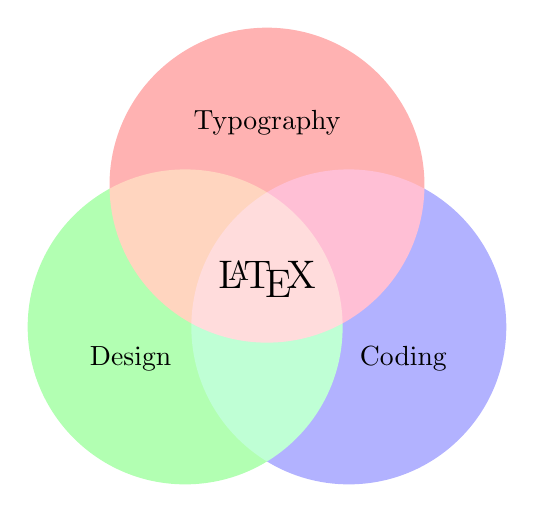
\begin{tikzpicture}
		\begin{scope}[blend group=soft light]
			\fill[red!30!white]   ( 90:1.2) circle (2);
			\fill[green!30!white] (210:1.2) circle (2);
			\fill[blue!30!white]  (330:1.2) circle (2);
		\end{scope}
		\node at ( 90:2) 	{Typography};
		\node at (210:2)  	{Design};
		\node at (330:2) {Coding};
		\node [font=\Large] {\LaTeX};
	\end{tikzpicture}
	\caption{Venn diagram TIKZ seg\'its\'egv\'evel}
\end{figure}

\begin{definition}
	Legyen $\left(X,d\right)$ \'es $\left(Y,\rho\right)$ k\'et metrikus
	t\'er, legyen $T:X\to Y$ egy lek\'epez\'es. Azt mondjuk, hogy a $T$ lek\'epez\'es
	Lipschitz tulajdons\'ag\'u, ha l\'etezik egy olyan $L>0$ sz\'am amelyre 
	\[
	\rho\left(Tx,Ty\right)\leq Ld(x,y)\;\forall x,y\in X.
	\]
	Az L sz\'amot Lipschitz \'alland\'onak nevezz\"uk.
\end{definition}

\pagebreak
Ha $T:X\to Y$ lek\'epez\'es Lipschitz tulajdons\'ag\'u, \'es az $L<1$ akkor
a $T$ oper\'atort \textbf{kontrakci\'onak} nevezz\"uk. Azt mondjuk, hogy
$x^{*}\in X$ fixpontja a $T$ oper\'atornak ha 
\[
Tx^{*}=x^{*}.
\]
\begin{theorem}{Banach f\'ele fixpontt\'etel}
	Legyen $\left(X,d\right)$ teljes metrikus t\'er \'es $T:X\to X$ lek\'epez\'es
	egy kontrakci\'o az $L<1$ \'alland\'oval. Ekkor igazak a k\"ovetkez\H{o}
	\'all\'it\'asok:
	\begin{enumerate}
		\item $T$-nek egy \'es csakis egy $x^{*}$ fixpontja.
		\item B\'arhogy v\'alasztunk meg egy $x_{0}\in X$ elemet, a $x_{k+1}=Tx_{k}$
		sorozat konvergens \'es $Tx_{k}\to x^{*},$ ahol $k$ term\'eszetes sz\'am.
		\item Igaz, hogy 
		\[
		d\left(x_{k},x^{*}\right)\leq\frac{L^{k}}{1-L}d(x_{0},Tx_{0}).
		\]
	\end{enumerate}
\end{theorem}
	%----------------------------------------------------------------------------
\chapter*{Összefoglaló}\addcontentsline{toc}{chapter}{Összefoglaló}
%----------------------------------------------------------------------------

...\\ \\

\url{https://github.com/bencekovacs01/F1_Ticket_Manager}

\url{https://github.com/bencekovacs01/F1_Ticket_Manager-NodeJS}

% Koszonetnyilvanitas
%~~~~~~~~~~~~~~~~~~~~~~~~~~~~~~~~~~~~~~~~~~~~~~~~~~~~~~~~~~~~~~~~~~~~~~~~~~~~~~~~~~~~~~
	%----------------------------------------------------------------------------
\chapter*{\koszonetnyilvanitas}\addcontentsline{toc}{chapter}{\koszonetnyilvanitas}
%----------------------------------------------------------------------------

Ez nem kötelező, akár törölhető is. Ha a szerző szükségét érzi, itt lehet köszönetet nyilvánítani azoknak, akik hozzájárultak munkájukkal ahhoz, hogy a hallgató a szakdolgozatban vagy diplomamunkában leírt feladatokat sikeresen elvégezze. A konzulensnek való köszönetnyilvánítás sem kötelező, a konzulensnek hivatalosan is dolga, hogy a hallgatót konzultálja.


% Tablazatok es abrak jegyzeke (EZ NEM KOTELEZO)
%~~~~~~~~~~~~~~~~~~~~~~~~~~~~~~~~~~~~~~~~~~~~~~~~~~~~~~~~~~~~~~~~~~~~~~~~~~~~~~~~~~~~~~
	\listoffigures\addcontentsline{toc}{chapter}{\abrakjegyzeke}
	\listoftables\addcontentsline{toc}{chapter}{\tablazatokjegyzeke}


% Bibliography
%~~~~~~~~~~~~~~~~~~~~~~~~~~~~~~~~~~~~~~~~~~~~~~~~~~~~~~~~~~~~~~~~~~~~~~~~~~~~~~~~~~~~~~
	\bibliography{mybib}
	\addcontentsline{toc}{chapter}{\irodalomjegyzek}
	\bibliographystyle{alpha}
	
% Appendix
%~~~~~~~~~~~~~~~~~~~~~~~~~~~~~~~~~~~~~~~~~~~~~~~~~~~~~~~~~~~~~~~~~~~~~~~~~~~~~~~~~~~~~~
	%----------------------------------------------------------------------------
\appendix
%----------------------------------------------------------------------------
\chapter*{\fuggelek}\addcontentsline{toc}{chapter}{\fuggelek}
\setcounter{chapter}{6}  % a fofejezet-szamlalo az angol ABC 6. betuje (F) lesz
\setcounter{equation}{0} % a fofejezet-szamlalo az angol ABC 6. betuje (F) lesz
\numberwithin{equation}{section}
\numberwithin{figure}{section}
\numberwithin{lstlisting}{section}
%\numberwithin{tabular}{section}

%----------------------------------------------------------------------------
\section{A TeXstudio felülete}
%----------------------------------------------------------------------------
\begin{figure}[!ht]
\centering
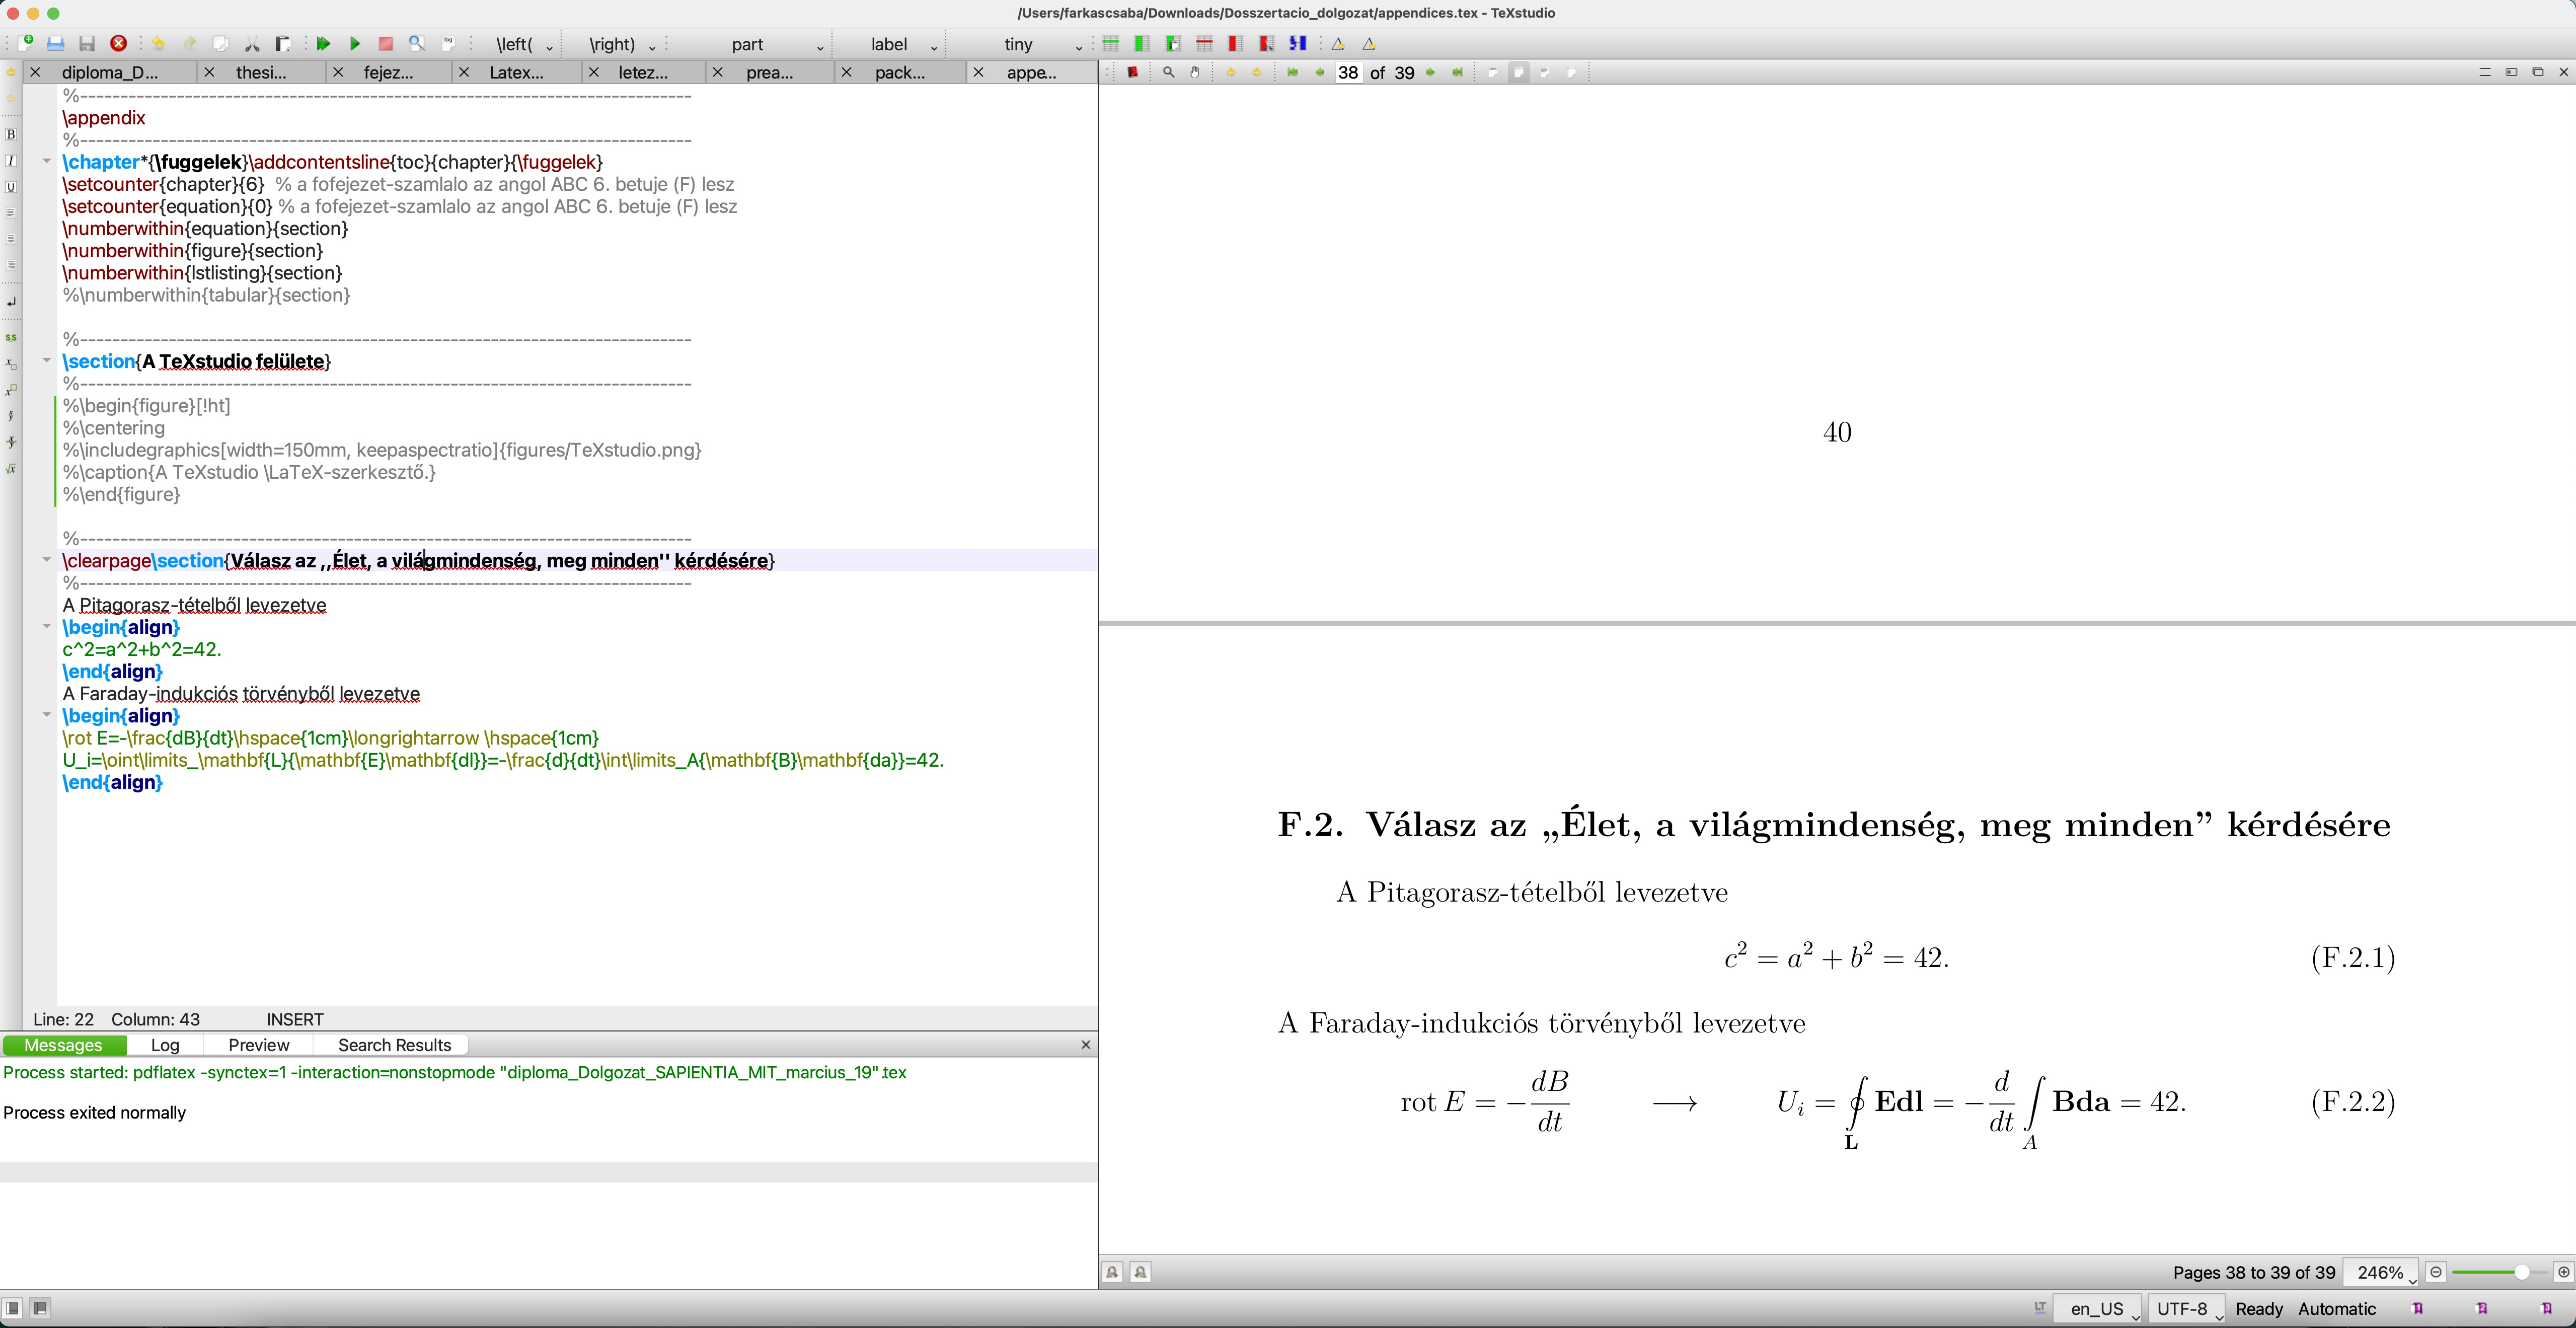
\includegraphics[width=150mm, keepaspectratio]{images/texstudio}
\caption{A TeXstudio \LaTeX-szerkesztő.} 
\end{figure}

%----------------------------------------------------------------------------
\clearpage\section{Válasz az ,,Élet, a világmindenség, meg minden'' kérdésére}
%----------------------------------------------------------------------------
A Pitagorasz-tételből levezetve
\begin{align}
c^2=a^2+b^2=42.
\end{align}
A Faraday-indukciós törvényből levezetve
\begin{align}
\rot E=-\frac{dB}{dt}\hspace{1cm}\longrightarrow \hspace{1cm}
U_i=\oint\limits_\mathbf{L}{\mathbf{E}\mathbf{dl}}=-\frac{d}{dt}\int\limits_A{\mathbf{B}\mathbf{da}}=42.
\end{align}







\label{page:last}
\end{document}
